\documentclass[sigconf,nonacm]{acmart}

\usepackage{amsmath}
\usepackage{array}
\usepackage{booktabs}
\usepackage{multirow}
\usepackage{tikz}
\usetikzlibrary{arrows.meta,positioning,fit,calc,shapes.geometric}
\usepackage{algorithm}
\usepackage{algpseudocode}

% Many floats in a two-column layout: give LaTeX room to queue them.
\extrafloats{100}

% Let pages hold more, and larger, figures and tables, so that floats pack
% together instead of each one opening a mostly empty page.
\setcounter{topnumber}{4}
\setcounter{bottomnumber}{2}
\setcounter{totalnumber}{6}
\setcounter{dbltopnumber}{4}
\renewcommand{\topfraction}{0.95}
\renewcommand{\bottomfraction}{0.8}
\renewcommand{\textfraction}{0.05}
\renewcommand{\floatpagefraction}{0.8}
\renewcommand{\dbltopfraction}{0.95}
\renewcommand{\dblfloatpagefraction}{0.8}

% Colour for the repository link under the abstract.
\definecolor{repoblue}{HTML}{1F5FBF}

% Scientific notation helper: \sci{6.68}{-16} -> 6.68 x 10^{-16}
\newcommand{\sci}[2]{\ensuremath{#1\times10^{#2}}}

% Group number, used in the subtitle.
\newcommand{\GroupNumber}{5}

\setcopyright{none}
\settopmatter{printacmref=false, printccs=true, printfolios=true}
\renewcommand\footnotetextcopyrightpermission[1]{}
\pagestyle{plain}

\begin{document}

\title{Exact Parameter Identification in PET Pharmacokinetic Modeling Using the Irreversible Two Tissue Compartment Model}
\subtitle{CSE 402 Numerical Analysis, Simulation and Modeling --- Section A1, Group \GroupNumber}

\author{Tasnimul Islam Mahi (2105013)}
\affiliation{%
  \institution{Department of Computer Science and Engineering, Bangladesh University of Engineering and Technology}
  \city{Dhaka}
  \country{Bangladesh}}

\author{Mafruha Islam Aishi (2105022)}
\affiliation{%
  \institution{Department of Computer Science and Engineering, Bangladesh University of Engineering and Technology}
  \city{Dhaka}
  \country{Bangladesh}}

\author{Ridhwanul Islam (2105024)}
\affiliation{%
  \institution{Department of Computer Science and Engineering, Bangladesh University of Engineering and Technology}
  \city{Dhaka}
  \country{Bangladesh}}

\author{Ashrafur Rahman (2105025)}
\affiliation{%
  \institution{Department of Computer Science and Engineering, Bangladesh University of Engineering and Technology}
  \city{Dhaka}
  \country{Bangladesh}}

\author{Tanvir Liaquat Uday (2105026)}
\affiliation{%
  \institution{Department of Computer Science and Engineering, Bangladesh University of Engineering and Technology}
  \city{Dhaka}
  \country{Bangladesh}}

\renewcommand{\shortauthors}{Mahi et al.}

\begin{abstract}
Dynamic positron emission tomography (PET) estimates regional kinetic parameters from tissue time--activity curves, but conventional quantification also requires an arterial input function obtained through invasive blood sampling. We reproduce the numerical core of Holler, Morina, and Schramm's exact-identifiability analysis for the irreversible two-tissue compartment model using hand-written numerical methods. The implementation includes LU factorization with partial pivoting, Householder QR least squares, nonuniform Simpson integration, a seeded linear congruential random-number generator with Box--Muller and Poisson samplers, power and inverse-power iterations, an analytic 104-by-23 Jacobian, and an iteratively regularized Gauss--Newton method (IRGNM). The closed-form tissue model agrees with an independent Radau ODE solution to $1.73\times10^{-13}$, and the quadrature path agrees to $3.29\times10^{-10}$. In 65 accepted noiseless tissue-only fits, the four ratios $K_{1,\mathrm{est}}^i/K_{1,\mathrm{true}}^i$ coincide to a worst spread of $1.83\times10^{-8}$ although individual $K_1$ error reaches 127\%; adding one early plasma measurement reduces $|\zeta-1|$ to at most $1.73\times10^{-7}$. Correcting a stopping-rule scaling error and adopting the paper's per-setup settings cut Monte Carlo blow-ups from 494 to 43 and match the paper's failure counts at high and normal count. With noise, the signature remains visible at high and normal count but fails at low count. Regularization reduces fitted-parameter variance by factors of 1.76 and 4.39. These results reproduce the paper's structural conclusion while exposing limits caused by TAC-level noise, initialization, stopping conventions, and floating-point evaluation.

\par\smallskip\noindent
\textbf{Code:}~\href{https://github.com/Undying2021Dreams/Numerical-Sessional-Project}{\textcolor{repoblue}{\nolinkurl{github.com/Undying2021Dreams/Numerical-Sessional-Project}}}
\end{abstract}

\begin{CCSXML}
<ccs2012>
 <concept>
  <concept_id>10002950.10003705.10003707</concept_id>
  <concept_desc>Mathematics of computing~Numerical analysis</concept_desc>
  <concept_significance>500</concept_significance>
 </concept>
 <concept>
  <concept_id>10002950.10003648.10003671</concept_id>
  <concept_desc>Mathematics of computing~Probabilistic algorithms</concept_desc>
  <concept_significance>300</concept_significance>
 </concept>
 <concept>
  <concept_id>10002950.10003714.10003715</concept_id>
  <concept_desc>Mathematics of computing~Numerical optimization</concept_desc>
  <concept_significance>300</concept_significance>
 </concept>
</ccs2012>
\end{CCSXML}

\ccsdesc[500]{Mathematics of computing~Numerical analysis}
\ccsdesc[300]{Mathematics of computing~Probabilistic algorithms}
\ccsdesc[300]{Mathematics of computing~Numerical optimization}

\keywords{dynamic PET, pharmacokinetic modeling, identifiability, inverse problems, IRGNM, regularization, numerical analysis, Monte Carlo simulation}

\maketitle

\section{Introduction and Base Paper Review}

Dynamic PET records tracer concentration over time and uses a compartment model to infer physiological rates. For an irreversible tracer, the regional parameters $K_1$, $k_2$, and $k_3$ respectively describe transport from plasma into tissue, return from tissue to plasma, and irreversible trapping. Clinical estimation normally depends on the metabolite-corrected arterial plasma concentration $C_P(t)$. Directly measuring that curve requires repeated blood draws and chemical processing; image-derived measurements more naturally provide whole-blood concentration $C_{WB}(t)$.

Holler, Morina, and Schramm~\cite{holler2024} analyzed simultaneous fitting of several regions under the irreversible two-tissue compartment model. Their main result states that, subject to technical assumptions and sufficiently many time samples, tissue observations identify every $k_2^i$ and $k_3^i$ and identify all $K_1^i$ up to one common scale. Blood information removes that scale ambiguity. They connect the noiseless theorem to noisy observations through Tikhonov regularization and an iteratively regularized Gauss--Newton method (IRGNM).

Our objective is not to reproduce the paper's digits. Its full simulation includes a sinogram and OSEM reconstruction chain, whereas ours adds calibrated noise directly to regional time--activity curves (TACs). Agreement is therefore defined \emph{before inspecting the results} as reproduction of mathematical invariants and qualitative trends: the common $K_1$ scale in tissue-only fitting, removal of that ambiguity by arterial information, decreasing error with decreasing noise, and reduced variance under regularization. Absolute failure counts are reported but are not expected to match.

The main contributions are: (i) a from-scratch numerical stack with no library solvers in the production modules, each component benchmarked against an independent reference; (ii) three independent evaluations of the forward model; (iii) an analytic Jacobian and regularized nonlinear solver; (iv) a 960-cell Monte Carlo study; (v) a direct parameter-level experiment for the paper's identifiability theorem; (vi) a record of the numerical enhancements we tried, including the ones that did not reach the final pipeline; and (vii) a controlled before-and-after evaluation of each improvement (Section~\ref{sec:improvements}). The public implementation and all regeneration scripts are available at \url{https://github.com/Undying2021Dreams/Numerical-Sessional-Project}.

\section{Methodology}

\subsection{Irreversible two-tissue model}

Figure~\ref{fig:compartment} shows the model. For each region, the exchangeable and trapped tissue compartments satisfy
\begin{align}
  \dot C_1(t) &= K_1 C_P(t)-(k_2+k_3)C_1(t), \\
  \dot C_2(t) &= k_3 C_1(t), \qquad C_T(t)=C_1(t)+C_2(t).
\end{align}
Writing $a=k_2+k_3$, the tissue concentration is evaluated as
\begin{equation}
C_T(t)=K_1\frac{k_2}{a}\int_0^t e^{-a(t-s)}C_P(s)\,ds
       +K_1\frac{k_3}{a}\int_0^t C_P(s)\,ds .
\label{eq:ct}
\end{equation}
The first term is a fading memory of recent input (the free compartment); the second is a running total of everything ever delivered, scaled by the trapping fraction $k_3/a$. The shared arterial input is a degree-four polyexponential,
\begin{equation}
C_P(t)=\sum_{j=1}^{4}\lambda_j e^{\mu_jt},
\label{eq:cp}
\end{equation}
and the parent-plasma fraction is
$f(t)=A e^{\xi_1t}+(1-A)e^{\xi_2t}$, giving
$C_{WB}=C_P/f$. The measured PET activity is
$C_{PET}=(1-V_B)C_T+V_BC_{WB}$ with $V_B=0.05$.

\begin{figure}[t]
  \centering
  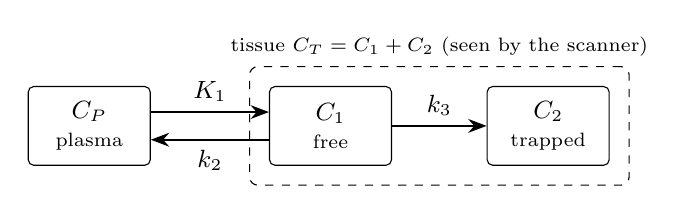
\begin{tikzpicture}[
      >=Stealth,
      comp/.style={draw, rounded corners=2pt, minimum width=1.55cm, minimum height=1.0cm, align=center, font=\small},
      lab/.style={font=\small}]
    \node[comp] (cp) {$C_P$\\[-1pt]{\scriptsize plasma}};
    \node[comp, right=1.5cm of cp] (c1) {$C_1$\\[-1pt]{\scriptsize free}};
    \node[comp, right=1.2cm of c1] (c2) {$C_2$\\[-1pt]{\scriptsize trapped}};
    \draw[->, thick] ([yshift=5pt]cp.east) -- node[lab, above] {$K_1$} ([yshift=5pt]c1.west);
    \draw[->, thick] ([yshift=-5pt]c1.west) -- node[lab, below] {$k_2$} ([yshift=-5pt]cp.east);
    \draw[->, thick] (c1.east) -- node[lab, above] {$k_3$} (c2.west);
    \node[draw, dashed, rounded corners=3pt, inner sep=7pt, fit=(c1)(c2),
          label={[font=\scriptsize]above:tissue $C_T=C_1+C_2$ (seen by the scanner)}] {};
  \end{tikzpicture}
  \caption{Irreversible two-tissue compartment model for one region. Tracer enters tissue at rate $K_1$, returns to plasma at $k_2$, and is trapped at $k_3$; trapped tracer never leaves.}
  \Description{Three boxes: plasma, free and trapped. Arrows K1 from plasma to free, k2 from free back to plasma, k3 from free to trapped. A dashed box around free and trapped is labelled tissue.}
  \label{fig:compartment}
\end{figure}

The unknown vector contains 23 parameters: four $\lambda_j$, four $\mu_j$, three parameters of $f$, and $(K_1,k_2,k_3)$ for each of four brain regions. The 11 blood parameters are shared by all regions, while each region owns its three kinetic rates. Ground-truth constants and the 25-frame schedule are taken from the paper's Section~5.1 and Table~2 and stored once in \texttt{src/config.py}.

\subsection{Software architecture}

Figure~\ref{fig:architecture} shows how the hand-written primitives feed the model and the solver. Each box is a module under \texttt{src/}; every arrow is a real call dependency. No higher layer calls a library routine: when it needs a linear solve, an integral, an eigenvalue, or a random number, it calls the primitive layer.

\begin{figure*}[t]
  \centering
  \resizebox{0.97\textwidth}{!}{%
  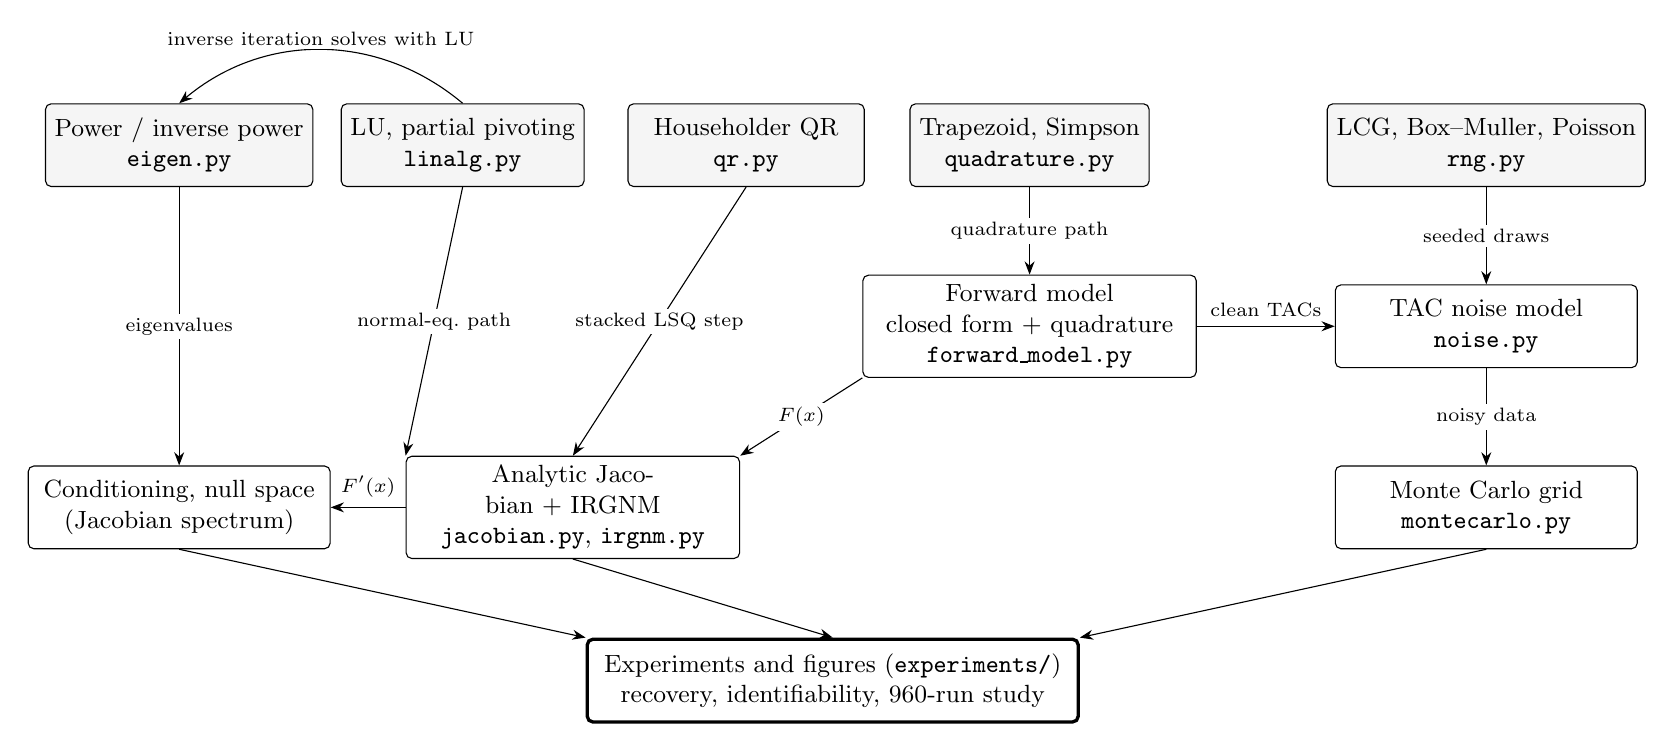
\begin{tikzpicture}[
      >=Stealth,
      prim/.style={draw, rounded corners=2pt, fill=gray!8, minimum width=3.0cm, minimum height=1.05cm, align=center, font=\small},
      mid/.style={draw, rounded corners=2pt, text width=3.6cm, minimum height=1.05cm, align=center, font=\small},
      top/.style={draw, rounded corners=2pt, very thick, text width=6.0cm, minimum height=1.05cm, align=center, font=\small},
      lab/.style={font=\scriptsize, fill=white, inner sep=1.5pt}]
    % Layer 1: primitives (ordered so that no arrows cross)
    \node[prim] (eig)  at (0,0)    {Power / inverse power\\\texttt{eigen.py}};
    \node[prim] (lu)   at (3.6,0)  {LU, partial pivoting\\\texttt{linalg.py}};
    \node[prim] (qr)   at (7.2,0)  {Householder QR\\\texttt{qr.py}};
    \node[prim] (quad) at (10.8,0) {Trapezoid, Simpson\\\texttt{quadrature.py}};
    \node[prim] (rng)  at (16.6,0) {LCG, Box--Muller, Poisson\\\texttt{rng.py}};
    % Layer 2: model
    \node[mid, text width=4.0cm] (fwd) at (10.8,-2.3) {Forward model\\closed form + quadrature\\\texttt{forward\_model.py}};
    \node[mid] (noise) at (16.6,-2.3) {TAC noise model\\\texttt{noise.py}};
    % Layer 3: solver and analysis
    \node[mid] (cond) at (0,-4.6)    {Conditioning, null space\\(Jacobian spectrum)};
    \node[mid, text width=4.0cm] (irg) at (5.0,-4.6) {Analytic Jacobian + IRGNM\\\texttt{jacobian.py}, \texttt{irgnm.py}};
    \node[mid] (mc)   at (16.6,-4.6) {Monte Carlo grid\\\texttt{montecarlo.py}};
    % Layer 4: experiments
    \node[top] (exp)  at (8.3,-6.8)  {Experiments and figures (\texttt{experiments/})\\recovery, identifiability, 960-run study};
    % Arrows
    \draw[->] (lu.north) to[bend right=40] node[lab, above]{inverse iteration solves with LU} (eig.north);
    \draw[->] (eig) -- node[lab]{eigenvalues} (cond);
    \draw[->] (lu.south) -- node[lab]{normal-eq.\ path} (irg.north west);
    \draw[->] (qr.south) -- node[lab]{stacked LSQ step} (irg.north);
    \draw[->] (quad) -- node[lab]{quadrature path} (fwd);
    \draw[->] (fwd.south west) -- node[lab]{$F(x)$} (irg.north east);
    \draw[->] (fwd.east) -- node[lab, above=2pt]{clean TACs} (noise.west);
    \draw[->] (rng) -- node[lab]{seeded draws} (noise);
    \draw[->] (irg.west) -- node[lab, above=2pt]{$F'(x)$} (cond.east);
    \draw[->] (noise) -- node[lab]{noisy data} (mc);
    \draw[->] (cond.south) -- (exp.north west);
    \draw[->] (irg.south) -- (exp.north);
    \draw[->] (mc.south) -- (exp.north east);
  \end{tikzpicture}}
  \caption{Module dependency graph. Shaded boxes are the hand-written primitives (Track A). The model, solver and experiment layers only reach numerical functionality through them; NumPy and SciPy appear only in tests and marked benchmarks (Track B).}
  \Description{Five primitive boxes in a top row (LU, QR, quadrature, random numbers, eigenvalues) feed a forward model and a noise model, which feed the Jacobian and IRGNM solver, the conditioning analysis and the Monte Carlo grid, which all feed the experiments box at the bottom.}
  \label{fig:architecture}
\end{figure*}

\subsection{Hand-written numerical primitives}

All production algorithms under \texttt{src/} are implemented without SciPy solvers, NumPy linear solves, or NumPy random sampling; NumPy is used only for array storage and elementwise arithmetic. An automated test walks the syntax tree of every module under \texttt{src/}, resolves import aliases, and fails on any banned symbol. This subsection describes each primitive in the form it is implemented.

\subsubsection{LU factorization with partial pivoting}
Linear systems $Ax=b$ are solved by Doolittle elimination with row pivoting, $PA=LU$, where $L$ is unit lower triangular and $U$ is upper triangular~\cite{golub2013,chapra2015}. At step $k$ the row with the largest $|a_{ik}|$, $i\ge k$, is swapped into the pivot position, so every multiplier satisfies $|\ell_{ik}|\le1$ and no division by a small pivot can amplify rounding error. A pivot below $10^{-300}$ in magnitude raises an explicit singular-matrix error instead of returning garbage. The solve is then two triangular sweeps, $Ly=Pb$ forward and $Ux=y$ backward (Algorithm~\ref{alg:lu}). The cost is $\tfrac23n^3$ flops for the factorization and $2n^2$ per right-hand side. LU is used inside inverse power iteration and in the normal-equations path of IRGNM that we keep for comparison.

\begin{algorithm}[t]
\caption{LU with partial pivoting (\texttt{lu\_factor}, \texttt{lu\_solve})}
\label{alg:lu}
\small
\begin{algorithmic}[1]
\Require $A\in\mathbb{R}^{n\times n}$, $b\in\mathbb{R}^n$
\For{$k=1$ \textbf{to} $n-1$}
  \State $p\gets\arg\max_{i\ge k}|a_{ik}|$; swap rows $k$ and $p$ of $A$; record $p$
  \If{$|a_{kk}|<10^{-300}$} \State \textbf{raise} singular matrix \EndIf
  \For{$i=k+1$ \textbf{to} $n$}
    \State $\ell_{ik}\gets a_{ik}/a_{kk}$ \Comment{$|\ell_{ik}|\le1$}
    \State $a_{i,k+1:n}\gets a_{i,k+1:n}-\ell_{ik}\,a_{k,k+1:n}$
  \EndFor
\EndFor
\State apply the recorded swaps to $b$
\State solve $Ly=b$ by forward substitution
\State solve $Ux=y$ by back substitution
\State \Return $x$
\end{algorithmic}
\end{algorithm}

\subsubsection{Householder QR and linear least squares}
For an $m\times n$ matrix with $m\ge n$, column $k$ is reduced by the reflector $H_k=I-2v_kv_k^T$ with
\begin{equation}
v_k=\frac{x-\alpha e_1}{\|x-\alpha e_1\|},\qquad \alpha=-\operatorname{sign}(x_1)\,\|x\|_2,
\label{eq:householder}
\end{equation}
where $x$ is the part of column $k$ on and below the diagonal (Algorithm~\ref{alg:qr}). Choosing the sign of $\alpha$ opposite to $x_1$ prevents cancellation in $x_1-\alpha$. The matrix $Q=H_1\cdots H_n$ is never formed: only the vectors $v_k$ are stored, and $Q^Tb$ is computed by re-applying them. For least squares, writing $Q^Tb=[c_1;c_2]$ gives the solution of $R_{1:n,1:n}x=c_1$ and the exact residual norm $\|c_2\|$. QR costs about twice as many flops as LU on a square system, but it works on $A$ directly instead of $A^TA$, so the condition number is not squared. This is why QR is the production solver inside IRGNM, and it is also the regression tool behind every log--log slope fit and the Patlak line in this report.

\begin{algorithm}[t]
\caption{Householder least squares (\texttt{qr\_factor}, \texttt{qr\_lstsq})}
\label{alg:qr}
\small
\begin{algorithmic}[1]
\Require $A\in\mathbb{R}^{m\times n}$ with $m\ge n$, $b\in\mathbb{R}^m$
\State $R\gets A$
\For{$k=1$ \textbf{to} $n$}
  \State $x\gets R_{k:m,k}$; \textbf{if} $\|x\|=0$ \textbf{then} store $v_k=0$ and continue
  \State $\alpha\gets-\operatorname{sign}(x_1)\|x\|_2$; $v\gets x-\alpha e_1$; $v_k\gets v/\|v\|$
  \State $R_{k:m,k:n}\gets R_{k:m,k:n}-2v_k\,(v_k^TR_{k:m,k:n})$
\EndFor
\State $c\gets b$; \textbf{for} $k=1$ \textbf{to} $n$: $c_{k:m}\gets c_{k:m}-2v_k(v_k^Tc_{k:m})$ \Comment{$c=Q^Tb$}
\State solve $R_{1:n,1:n}\,x=c_{1:n}$ by back substitution
\State \Return $x$ and residual norm $\|c_{n+1:m}\|$
\end{algorithmic}
\end{algorithm}

\subsubsection{Trapezoid and Simpson integration on nonuniform grids}
The composite trapezoid rule is $\sum_i \tfrac12(x_{i+1}-x_i)(y_i+y_{i+1})$, with error $O(h^2)$. Simpson's rule must also work on the nonuniform grids used by the forward model, so it is implemented by integrating the quadratic interpolant through each consecutive node triple $x_0<x_1<x_2$ exactly. With $h_0=x_1-x_0$, $h_1=x_2-x_1$ and $w=h_0+h_1$,
\begin{equation}
\int_{x_0}^{x_2}p_2\,dx=\frac{w}{6}\left[\Big(2-\frac{h_1}{h_0}\Big)y_0+\frac{w^2}{h_0h_1}\,y_1+\Big(2-\frac{h_0}{h_1}\Big)y_2\right],
\label{eq:simpson}
\end{equation}
which reduces to the textbook weights $\tfrac{h}{3}(1,4,1)$ when $h_0=h_1=h$. If the number of intervals is odd, the last interval is closed with one trapezoid step and the fallback is reported. On a uniform grid the leading error of the composite rule is
\begin{equation}
E(h)\approx\frac{h^4}{180}\big[f'''(b)-f'''(a)\big]+O(h^6),
\label{eq:simpsonerror}
\end{equation}
so halving $h$ divides the error by 16. When $f'''(a)=f'''(b)$ the $h^4$ term cancels and the observed order becomes 6; Section~\ref{sec:results-quad} shows this happening.

\subsubsection{Random numbers: LCG, Box--Muller and Poisson}
Uniform numbers come from a 64-bit linear congruential generator~\cite{knuth1997}
\begin{equation}
s_{k+1}=(a\,s_k+c)\bmod 2^{64},\qquad u_k=\lfloor s_{k+1}/2^{11}\rfloor\cdot2^{-53},
\label{eq:lcg}
\end{equation}
with Knuth's MMIX constants $a=6364136223846793005$ and $c=1442695040888963407$. Only the top 53 bits are used, because the low bits of an LCG have short periods, and 53 bits fill a float64 mantissa exactly. The integer seed is first passed through a SplitMix64 avalanche so that nearby seeds do not start in related states, and sub-seeds for each experiment are derived deterministically from a SHA-256 hash of the root seed and string labels. Normal variates use the Box--Muller transform~\cite{box1958},
\begin{equation}
z_1=\sqrt{-2\ln u_1}\cos(2\pi u_2),\qquad z_2=\sqrt{-2\ln u_1}\sin(2\pi u_2),
\label{eq:boxmuller}
\end{equation}
with $u_1$ drawn from the open interval $(0,1)$ so the logarithm stays finite. Poisson variates use Knuth's multiplication algorithm, which multiplies uniforms until the product drops below $e^{-\lambda}$, for $\lambda\le30$, and the rounded normal approximation $\max(0,\operatorname{round}(\lambda+\sqrt{\lambda}\,z))$ above it. The crossover matters: Knuth's method costs $O(\lambda)$ uniforms per draw, and for $\lambda\gtrsim745$ the threshold $e^{-\lambda}$ underflows to zero, so the loop would never terminate.

\subsubsection{Power and inverse power iteration}
The largest eigenvalue of the symmetric matrix $M=F'^TF'$ is found by the power method with a Rayleigh-quotient stopping test (relative change below $10^{-13}$), and the full spectrum by repeated Hotelling deflation $M\leftarrow M-\lambda vv^T$. The smallest eigenvalue, which sets the conditioning, comes from inverse power iteration, where each step solves $Mw=v$ with our LU factorization.

\subsection{Stable forward evaluation and quadrature}

Equation~\eqref{eq:ct} has both a closed-form and an independently integrated implementation. Substituting the polyexponential~\eqref{eq:cp} turns both integrals into sums of terms of the form $\int_0^te^{cs}\,ds=t\,\phi_1(ct)$, with
\begin{equation}
\phi_1(z)=\frac{e^z-1}{z},\qquad \phi_1(0)=1 .
\label{eq:phi1}
\end{equation}
Evaluated literally, $\phi_1$ subtracts two nearly equal numbers when $|z|$ is small, and at $z=0$ it is $0/0$. We evaluate it as \texttt{expm1(z)/z}, which computes $e^z-1$ without forming $e^z$ first. For one exponential component, the convolution kernel is evaluated as
\begin{equation}
E(t,a,\mu)=t\,e^{\max(\mu,-a)t}\,\phi_1(-|a+\mu|t),
\label{eq:stablekernel}
\end{equation}
which avoids an artificial $0\cdot\infty$ intermediate and stays finite when $a+\mu\to0$. The Jacobian needs $\phi_1'(x)=1+(x-1)\phi_2(x)$ with $\phi_2(x)=(e^x-1-x)/x^2$. Here \texttt{expm1} alone is not enough, because the numerator still subtracts $x$ from a nearly equal quantity; below $|x|=10^{-4}$, a threshold we measured rather than assumed, we switch to the Taylor series $\phi_2(x)=\tfrac12+\tfrac{x}{6}+\tfrac{x^2}{24}+\cdots$, whose terms are all added.

The independent path applies our nonuniform composite Simpson rule on a graded grid $t_i=t_{\max}u_i^3$ with $u_i$ uniform on $[0,1]$ and 1601 points. Grading places most nodes in the first minutes, where the injected bolus makes $C_P$ change fastest. Three-point Lagrange weights are computed in local coordinates, as in~\eqref{eq:simpson}. This change preserves Simpson's rule while avoiding cancellation from subtracting cubic antiderivatives at large absolute coordinates.

\subsection{Analytic Jacobian and IRGNM}

The forward operator $F:\mathbb{R}^{23}\rightarrow\mathbb{R}^{104}$ contains 100 regional TAC observations (4 regions times 25 frames) and four blood constraints $C_{WB}(s)f(s)-C_P(s)$ at the sampling times $s\in\{0.29,2.25,15,57.5\}$ min. Its analytic Jacobian is derived from the closed form and verified columnwise against central differences. The Jacobian is block structured: each region's rows depend on the shared blood parameters and on that region's own three rates only, the tissue rows do not depend on the plasma-fraction parameters, and the blood rows do not depend on any tissue rate. The regularization and globalization choices follow established inverse-problem and nonlinear-optimization principles~\cite{hansen2010,nocedal2006}. At iteration $i$, the IRGNM step solves
\begin{equation}
\min_{\Delta x}\left\|
\begin{bmatrix}F'(x_i)\\ \Lambda_i^{1/2}\end{bmatrix}\Delta x-
\begin{bmatrix}y^\delta-F(x_i)\\ \Lambda_i^{1/2}(x_0-x_i)\end{bmatrix}
\right\|_2^2,
\label{eq:irgnm}
\end{equation}
using Householder QR. Six blockwise regularization schedules follow $a e^{-bi}$: metabolic, arterial, and plasma-fraction blocks each have separate magnitudes, because the 23 parameters span a scale ratio of 2690. The adopted values are $a_\alpha=4000$, $a_\beta=100$, $a_\gamma=200$, $b=\ln(2)/7$, and discrepancy factor $\tau=6.8$. Each full step is projected onto the feasible domain. A normal-equations/LU path is retained for comparison; the production solver takes full steps without a line search. Figure~\ref{fig:irgnmflow} summarizes one run.

\begin{figure}[t]
  \centering
  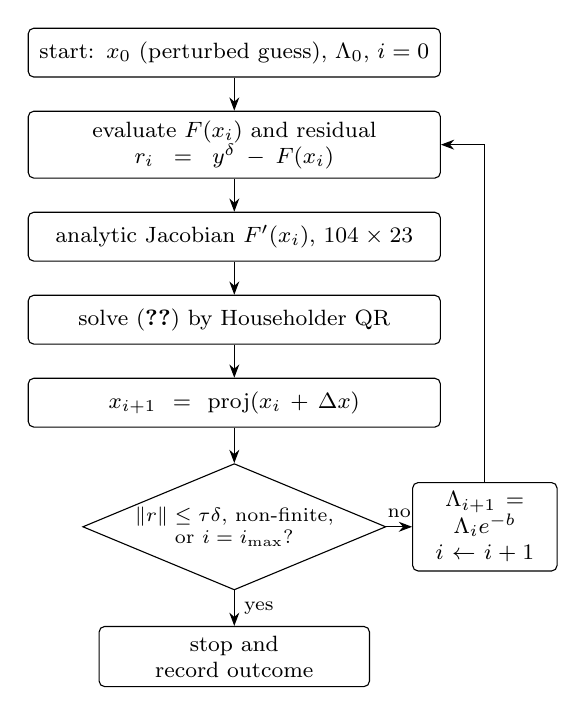
\begin{tikzpicture}[
      >=Stealth, node distance=0.42cm,
      blk/.style={draw, rounded corners=2pt, text width=5.0cm, minimum height=0.62cm, align=center, font=\footnotesize},
      dec/.style={draw, diamond, aspect=2.4, inner sep=0.5pt, align=center, font=\scriptsize}]
    \node[blk] (s0) {start: $x_0$ (perturbed guess), $\Lambda_0$, $i=0$};
    \node[blk, below=of s0] (s1) {evaluate $F(x_i)$ and residual\\$r_i=y^\delta-F(x_i)$};
    \node[blk, below=of s1] (s2) {analytic Jacobian $F'(x_i)$, $104\times23$};
    \node[blk, below=of s2] (s3) {solve~\eqref{eq:irgnm} by Householder QR};
    \node[blk, below=of s3] (s4) {$x_{i+1}=\mathrm{proj}(x_i+\Delta x)$};
    \node[dec, below=0.45cm of s4] (d) {$\|r\|\le\tau\delta$, non-finite,\\or $i=i_{\max}$?};
    \node[blk, below=0.45cm of d, text width=3.2cm] (stop) {stop and record outcome};
    \node[blk, text width=1.6cm] (shrink) at ($(d.east)+(1.25,0)$) {$\Lambda_{i+1}=\Lambda_ie^{-b}$\\$i\gets i+1$};
    \draw[->] (s0) -- (s1);
    \draw[->] (s1) -- (s2);
    \draw[->] (s2) -- (s3);
    \draw[->] (s3) -- (s4);
    \draw[->] (s4) -- (d);
    \draw[->] (d) -- node[right, font=\scriptsize]{yes} (stop);
    \draw[->] (d.east) -- node[above, font=\scriptsize]{no} (shrink.west);
    \draw[->] (shrink.north) |- (s1.east);
  \end{tikzpicture}
  \caption{One IRGNM run. The regularization weights shrink geometrically, so early steps are cautious and later steps approach plain Gauss--Newton. Divergence (non-finite iterates) is recorded as a failure, never silently retried.}
  \Description{A vertical flowchart: start, evaluate forward model and residual, build Jacobian, solve stacked least-squares problem by QR, project the step, then a decision diamond that either stops or shrinks the regularization and loops back to the evaluation step.}
  \label{fig:irgnmflow}
\end{figure}

For noisy data, Morozov stopping compares the residual 2-norm with $\tau$ times the noise 2-norm. Since calibration returns an RMS discrepancy $\delta_y$, experiments pass $\sqrt{n_{obs}}\,\delta_y$ where dimensionally required. Iteration-zero stops are recorded as trivial stops, not successful fits.

\subsection{Identifiability statistic}

With tissue data only, the transformation
\begin{equation}
K_1^i\mapsto \zeta K_1^i,\qquad
\lambda_j\mapsto \lambda_j/\zeta
\end{equation}
leaves every regional TAC unchanged. We measure
\begin{equation}
s_\zeta=\frac{\max_i(K_{1,\mathrm{est}}^i/K_{1,\mathrm{true}}^i)}
{\min_i(K_{1,\mathrm{est}}^i/K_{1,\mathrm{true}}^i)}-1.
\end{equation}
A small $s_\zeta$ together with a large $|\zeta-1|$ is the predicted signature. We then restore a single $C_P$ observation and measure the collapse of $|\zeta-1|$.

\section{Implementation and Experiments}

\subsection{Synthetic data and measurement setups}

The four regions are frontal, temporal, occipital, and white matter. Their ground-truth $(K_1,k_2,k_3)$ values, taken from the base paper~\cite{holler2024}, are the control-group values of Jagust et al.~\cite{jagust1991}: $(0.157,0.174,0.118)$, $(0.161,0.179,0.096)$, $(0.177,0.159,0.088)$, and $(0.100,0.161,0.047)$. The acquisition contains 25 frames: $4\times5$ s, $4\times10$ s, $4\times30$ s, $2\times60$ s, $3\times150$ s, $6\times300$ s, and $2\times600$ s. Figure~\ref{fig:forward} shows the resulting curves.

\begin{figure*}[t]
  \centering
  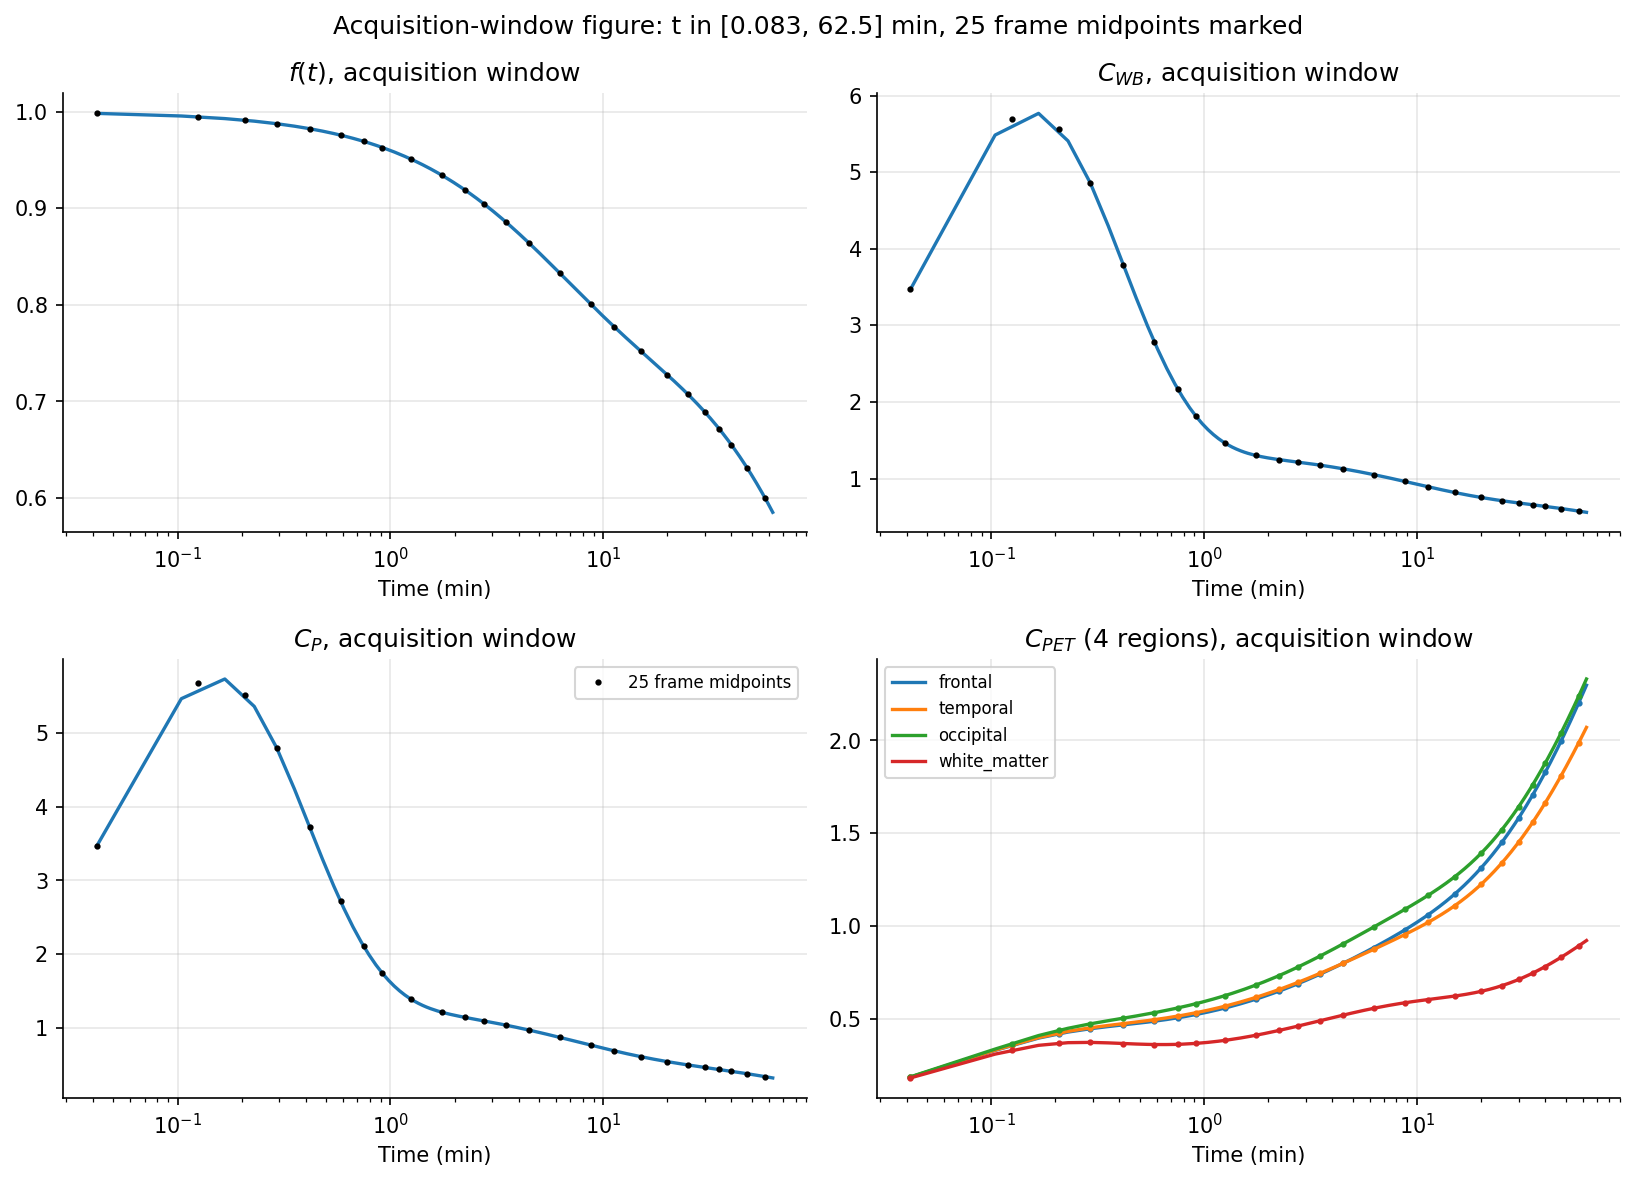
\includegraphics[width=0.94\textwidth]{figures/figure2_acquisition_window.png}
  \caption{Synthetic plasma fraction, whole-blood input, plasma input, and four regional PET TACs over the 25-frame acquisition window. Dots mark frame midpoints.}
  \Description{Four panels show a decreasing plasma fraction, peaked whole-blood and plasma input curves, and increasing regional PET time-activity curves.}
  \label{fig:forward}
\end{figure*}

Poisson-derived TAC noise and Gaussian blood noise were calibrated by bisection to target RMS discrepancies $0.003$, $0.011$, and $0.070$ for high, normal, and low count. The experiment grid contains three setups, four noise levels (including noiseless), four initial perturbation levels $\delta_x\in\{0.1,0.2,0.3,0.4\}$, and 20 deterministic seeds: 960 fits. Setup A fixes the plasma-fraction parameters and omits the blood block; Setup B fits all 23 parameters with clean $C_{WB}$; Setup C fits all parameters with noisy $C_{WB}$. This repository's Setup A is therefore the deliberately tissue-only identifiability configuration and is not numerically identical to every setting in the paper's Table~1.

\subsection{Benchmarks for the numerical building blocks}

Every primitive is tested against a truth that is known independently of the code under test (Table~\ref{tab:benchsetup}). For linear systems we use manufactured solutions: we choose $x$, form $b=Ax$, and compare the computed $x$ with the chosen one, with NumPy as a second referee. The Hilbert matrices $H_{ij}=1/(i+j+1)$ with $x=(1,\dots,1)$ are a deliberately ill-conditioned stress test. Integration is checked on integrals with known values, the random generators against the moments and distribution functions of their target laws, and the forward model against two independent code paths. Convergence orders are measured as least-squares slopes on log--log data, computed with our own QR routine.

\begin{table*}[t]
\caption{Benchmark design for the numerical building blocks and the scripts that regenerate them.}
\label{tab:benchsetup}
\small
\begin{tabular}{p{0.14\textwidth}p{0.40\textwidth}p{0.18\textwidth}p{0.18\textwidth}}
\toprule
Component & Test design & Independent truth & Script \\
\midrule
LU, QR & 200 random systems, $n=5$ to 100; Hilbert $n=6,8,10,12$ & manufactured $x$; NumPy & \texttt{m1\_linalg\_benchmark.py} \\
Trapezoid, Simpson & $\int_0^\pi\sin x$, $\int_0^1e^x$, $\int_0^1(1+x^2)^{-1}$; $n=9$ to 2001 points & exact values $2$, $e-1$, $\pi/4$ & \texttt{m1\_quadrature\_benchmark.py} \\
RNG & $10^6$ uniforms and normals (seed 123); $2\times10^5$ Poisson draws per $\lambda$ & theoretical moments, $\chi^2$, $\Phi$ & \texttt{m1\_rng\_benchmark.py} \\
Forward model & all 4 regions, all 25 frames; $\phi_1$ sweep; grid refinement; Patlak fit & Radau and RK45 ODE solvers & \texttt{m2\_forward\_model.py} \\
Jacobian, conditioning & central differences, relative step $1.5\times10^{-5}$; full spectrum & finite differences; NumPy eigenvalues & \texttt{m3\_jacobian\_and\_solver.py} \\
IRGNM recovery & 20 seeds per $\delta_x$, 300 iterations, noiseless data & hidden ground truth & \texttt{m3\_irgnm\_recovery.py} \\
\bottomrule
\end{tabular}
\end{table*}

\subsection{Verification protocol}

Track A denotes the hand-written implementation; Track B denotes NumPy~\cite{harris2020} and SciPy~\cite{virtanen2020} used only as independent benchmarks in \texttt{tests/} or \texttt{experiments/}. The forward model was checked against direct Simpson integration and \texttt{solve\_ivp} with the implicit Radau method. The Jacobian was checked against central differences. Figures are generated with Matplotlib~\cite{hunter2007}, and the experiment harness runs on Python~\cite{python2026}. Every stochastic run uses a derived seed, and generated JSON files record the root seed, configuration hash, source hash, Python/NumPy versions, and platform. The primary numerical artifacts use configuration hash \texttt{2f38ba062972} and source-hash prefix \texttt{9d11616d97b7}. The latest one-command manifest records 18 of 18 scripts completing successfully in 2264.7 s on Windows with Python 3.10.6 and NumPy 2.2.6. A fresh full test run reports 176 passed; the solver-ban guard remains part of that suite.

\section{Results and Discussion}

\subsection{Numerical verification}

Table~\ref{tab:verification} shows that the numerical building blocks reach the accuracy needed by the inverse problem. The analytic closed form is effectively indistinguishable from the independent stiff ODE reference. The graded-grid quadrature is less accurate but remains below $3.30\times10^{-10}$ relative difference across all four regions and 25 frames. The following subsections give the detail behind each row.

\begin{table}[t]
\caption{Verification summary for the hand-written numerical stack.}
\label{tab:verification}
\small
\begin{tabular}{p{0.39\columnwidth}p{0.52\columnwidth}}
\toprule
Component & Measured result \\
\midrule
LU vs NumPy, 200 systems & max relative error $6.48\times10^{-16}$ \\
QR vs NumPy, 200 systems & max relative error $1.13\times10^{-15}$ \\
Trapezoid order & $1.9999$--$2.0008$ \\
Simpson order & $3.9987$ and $4.0125$; $5.9988$ for a cancellation case \\
Closed form vs Radau & $1.73\times10^{-13}$ \\
Quadrature vs Radau & $3.29\times10^{-10}$ \\
Jacobian vs finite differences & $3.62\times10^{-6}$ ($\lambda$), $1.72\times10^{-6}$ ($\mu$), $1.27\times10^{-7}$ ($m$), $2.85\times10^{-8}$ (kinetics) \\
Power method, largest eigenvalue & $22320.478409382842$ vs $22320.478409382828$ \\
\bottomrule
\end{tabular}
\end{table}

\subsubsection{Linear solvers}
On 200 random systems of size 5 to 100, the mean relative residual $\|Ax-b\|/\|b\|$ is \sci{2.67}{-16} for LU and \sci{5.51}{-16} for QR, with maxima \sci{4.65}{-16} and \sci{9.22}{-16} (Figure~\ref{fig:linalg}). Both are at the level of the unit round-off $\approx\sci{1.1}{-16}$, so neither solver loses accuracy as $n$ grows. QR's mean residual is about twice LU's, consistent with its roughly doubled operation count.

\begin{figure}[t]
  \centering
  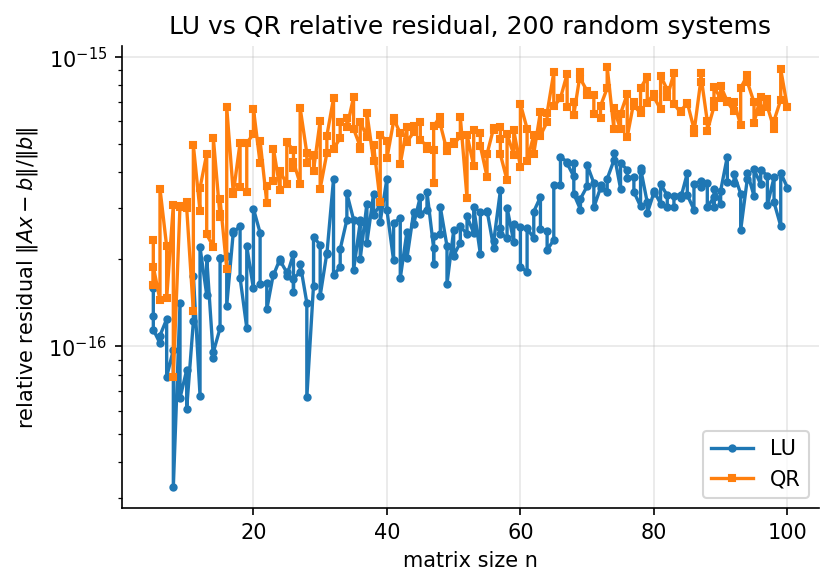
\includegraphics[width=\columnwidth]{figures/linalg_residuals.png}
  \caption{Relative residual of our LU and QR solvers on 200 random systems of size 5 to 100. Both stay below $10^{-15}$ at every size.}
  \Description{Two noisy lines against matrix size: LU between about 3e-17 and 5e-16, QR between about 1e-16 and 1e-15, both roughly flat.}
  \label{fig:linalg}
\end{figure}

Table~\ref{tab:hilbert} shows the Hilbert stress test. Here the residual stays tiny but the error in $x$ grows with the condition number, following the rule of thumb that about $\log_{10}\kappa(A)$ of the 16 available decimal digits are lost. At $n=12$, $\kappa\approx\sci{1.8}{16}$ leaves at most one or two correct digits, and LU, QR and NumPy all fail, by different amounts. This is a property of the matrix, not of any implementation, and it is the same mechanism that makes the parameter-identification problem need regularization.

\begin{table}[t]
\caption{Hilbert systems with exact solution $x=(1,\dots,1)$: relative error of the computed solution.}
\label{tab:hilbert}
\footnotesize
\setlength{\tabcolsep}{4pt}
\begin{tabular}{ccccc}
\toprule
$n$ & $\kappa_2(H)$ & LU & QR & NumPy \\
\midrule
6  & \sci{1.50}{7}  & \sci{2.54}{-10} & \sci{4.25}{-11} & \sci{1.42}{-10} \\
8  & \sci{1.53}{10} & \sci{1.20}{-7}  & \sci{1.93}{-7}  & \sci{6.12}{-8} \\
10 & \sci{1.60}{13} & \sci{2.68}{-4}  & \sci{2.13}{-4}  & \sci{8.67}{-5} \\
12 & \sci{1.76}{16} & \sci{3.91}{-2}  & \sci{1.73}{-1}  & \sci{3.25}{-1} \\
\bottomrule
\end{tabular}
\end{table}

\subsubsection{Integration}
\label{sec:results-quad}
Halving the step must divide the trapezoid error by $2^2=4$ and the Simpson error by $2^4=16$. Table~\ref{tab:quadratio} shows exactly this for $\int_0^\pi\sin x\,dx=2$; the fitted orders are 2.0008 and 4.0125. For $e^x$ on $[0,1]$ they are 1.9999 and 3.9987. For $f(x)=1/(1+x^2)$ on $[0,1]$, Simpson measures order 5.9988: here $f'''(x)=24x(1-x^2)/(1+x^2)^4$ vanishes at both endpoints, so the $h^4$ term of~\eqref{eq:simpsonerror} cancels and the $h^6$ term is what we see. With local-coordinate weights the Simpson error keeps falling to \sci{6.6}{-14} at $n=2001$ for $\sin x$ and reaches the float64 limit (\sci{2.2}{-16}) for the cancellation case (Figure~\ref{fig:quadrature}).

\begin{table}[t]
\caption{Error of $\int_0^\pi\sin x\,dx$ as the grid is refined. The ratio is the error at the previous $n$ divided by the error at this $n$.}
\label{tab:quadratio}
\small
\begin{tabular}{rcccc}
\toprule
$n$ & trapezoid error & ratio & Simpson error & ratio \\
\midrule
9    & \sci{2.58}{-2} & ---  & \sci{2.69}{-4}  & ---   \\
17   & \sci{6.43}{-3} & 4.01 & \sci{1.66}{-5}  & 16.23 \\
33   & \sci{1.61}{-3} & 4.00 & \sci{1.03}{-6}  & 16.06 \\
65   & \sci{4.02}{-4} & 4.00 & \sci{6.45}{-8}  & 16.01 \\
129  & \sci{1.00}{-4} & 4.00 & \sci{4.03}{-9}  & 16.00 \\
257  & \sci{2.51}{-5} & 4.00 & \sci{2.52}{-10} & 16.00 \\
513  & \sci{6.27}{-6} & 4.00 & \sci{1.57}{-11} & 16.00 \\
1025 & \sci{1.57}{-6} & 4.00 & \sci{9.85}{-13} & 15.98 \\
\bottomrule
\end{tabular}
\end{table}

\begin{figure*}[t]
  \centering
  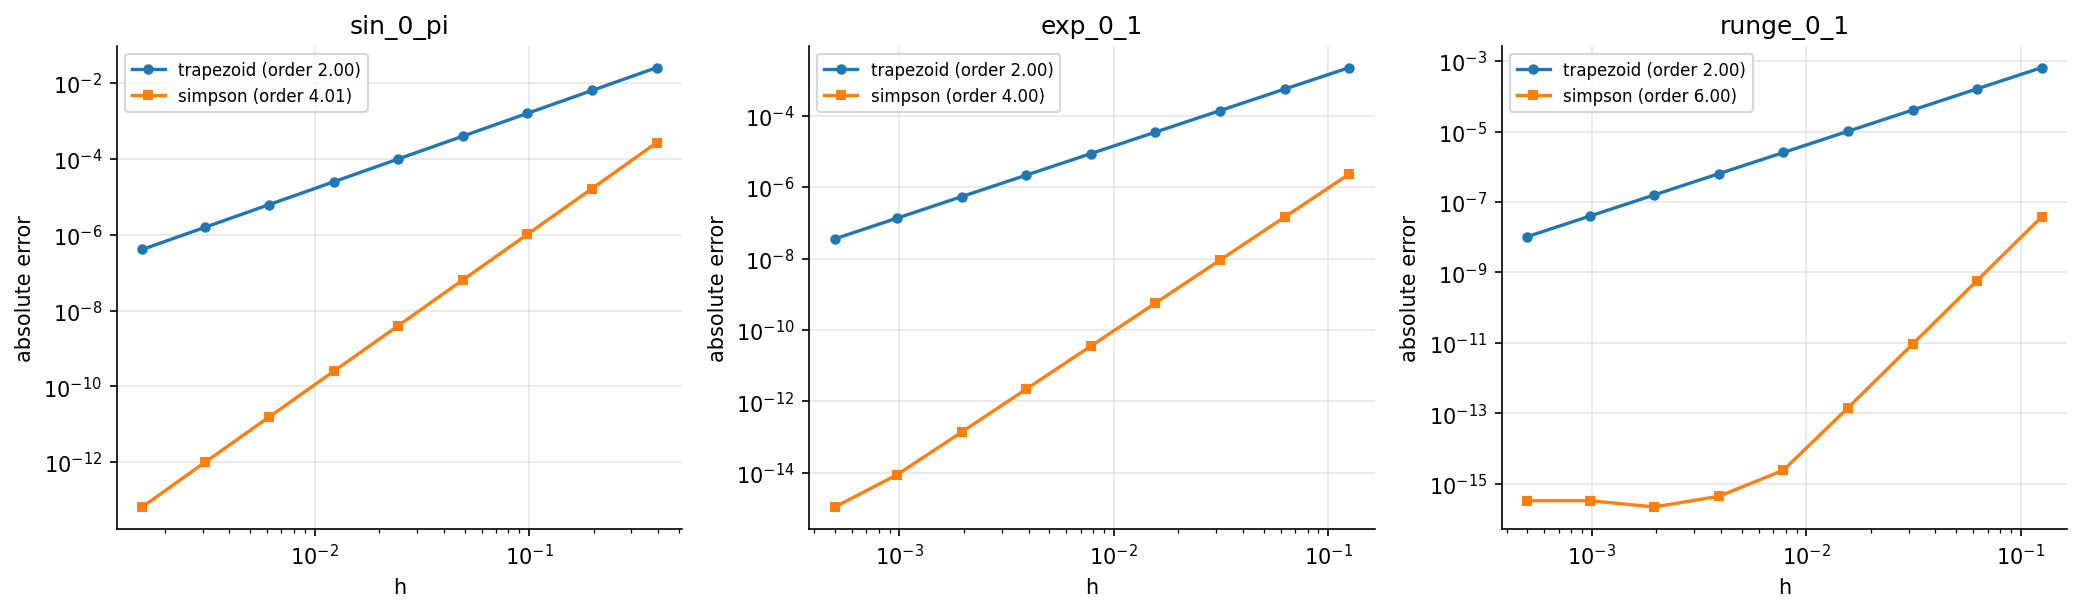
\includegraphics[width=0.96\textwidth]{figures/quadrature_convergence.png}
  \caption{Absolute error against step size $h$ on log--log axes; the slope is the convergence order. Trapezoid has slope 2 and Simpson slope 4, except for $(1+x^2)^{-1}$, where the endpoint cancellation in~\eqref{eq:simpsonerror} gives slope 6 until the error reaches machine precision.}
  \Description{Three log-log panels for sin, exp and 1/(1+x^2). Trapezoid lines have slope 2; Simpson lines have slope 4, and slope 6 in the third panel before flattening near 1e-15.}
  \label{fig:quadrature}
\end{figure*}

\subsubsection{Random numbers}
Table~\ref{tab:rng} summarizes the generator diagnostics. The uniform stream has the theoretical mean and variance to four digits. A chi-square test over 10 equal bins of $10^6$ draws gives 12.68, below the 5\% critical value 16.92 for 9 degrees of freedom, so uniformity is not rejected. The Box--Muller normals have mean, skewness and excess kurtosis near 0 and variance near 1, and their empirical distribution function stays within \sci{5.6}{-4} of $\Phi$ on $[-3,3]$. Lag-1 to lag-5 autocorrelations of the uniform stream all lie inside one standard error ($1/\sqrt{n}=10^{-3}$) of zero. That matters because Box--Muller is known to expose correlations between consecutive LCG outputs (the Neave effect). Both Poisson branches reproduce mean $=$ variance $=\lambda$ within Monte Carlo error. Figure~\ref{fig:rng} shows the histograms and the consecutive-pair scatters; the uniform pairs fill the square without the lattice stripes of a poor LCG.

\begin{table}[t]
\caption{Random-number diagnostics ($n=10^6$ unless stated).}
\label{tab:rng}
\footnotesize
\begin{tabular}{p{0.40\columnwidth}p{0.30\columnwidth}p{0.20\columnwidth}}
\toprule
Statistic & Measured & Target \\
\midrule
Uniform mean / variance & 0.499721 / 0.083412 & 0.5 / 0.083333 \\
$\chi^2$, 10 bins, 9 d.o.f. & 12.68 & $<16.92$ (5\%) \\
Normal mean / variance & 0.000388 / 1.000037 & 0 / 1 \\
Normal skew / excess kurtosis & 0.0035 / 0.0038 & 0 / 0 \\
$\max|\hat F-\Phi|$ on $[-3,3]$ & \sci{5.6}{-4} & $\to0$ \\
Autocorrelation, lags 1--5 & $|\rho|\le\sci{4.0}{-4}$ & $|\rho|<10^{-3}$ \\
Poisson $\lambda=4$ (Knuth) & 4.0013 / 4.0046 & 4 / 4 \\
Poisson $\lambda=25$ (Knuth) & 24.991 / 25.012 & 25 / 25 \\
Poisson $\lambda=1000$ (normal) & 1000.004 / 1002.29 & 1000 / 1000 \\
\bottomrule
\end{tabular}
\end{table}

\begin{figure*}[t]
  \centering
  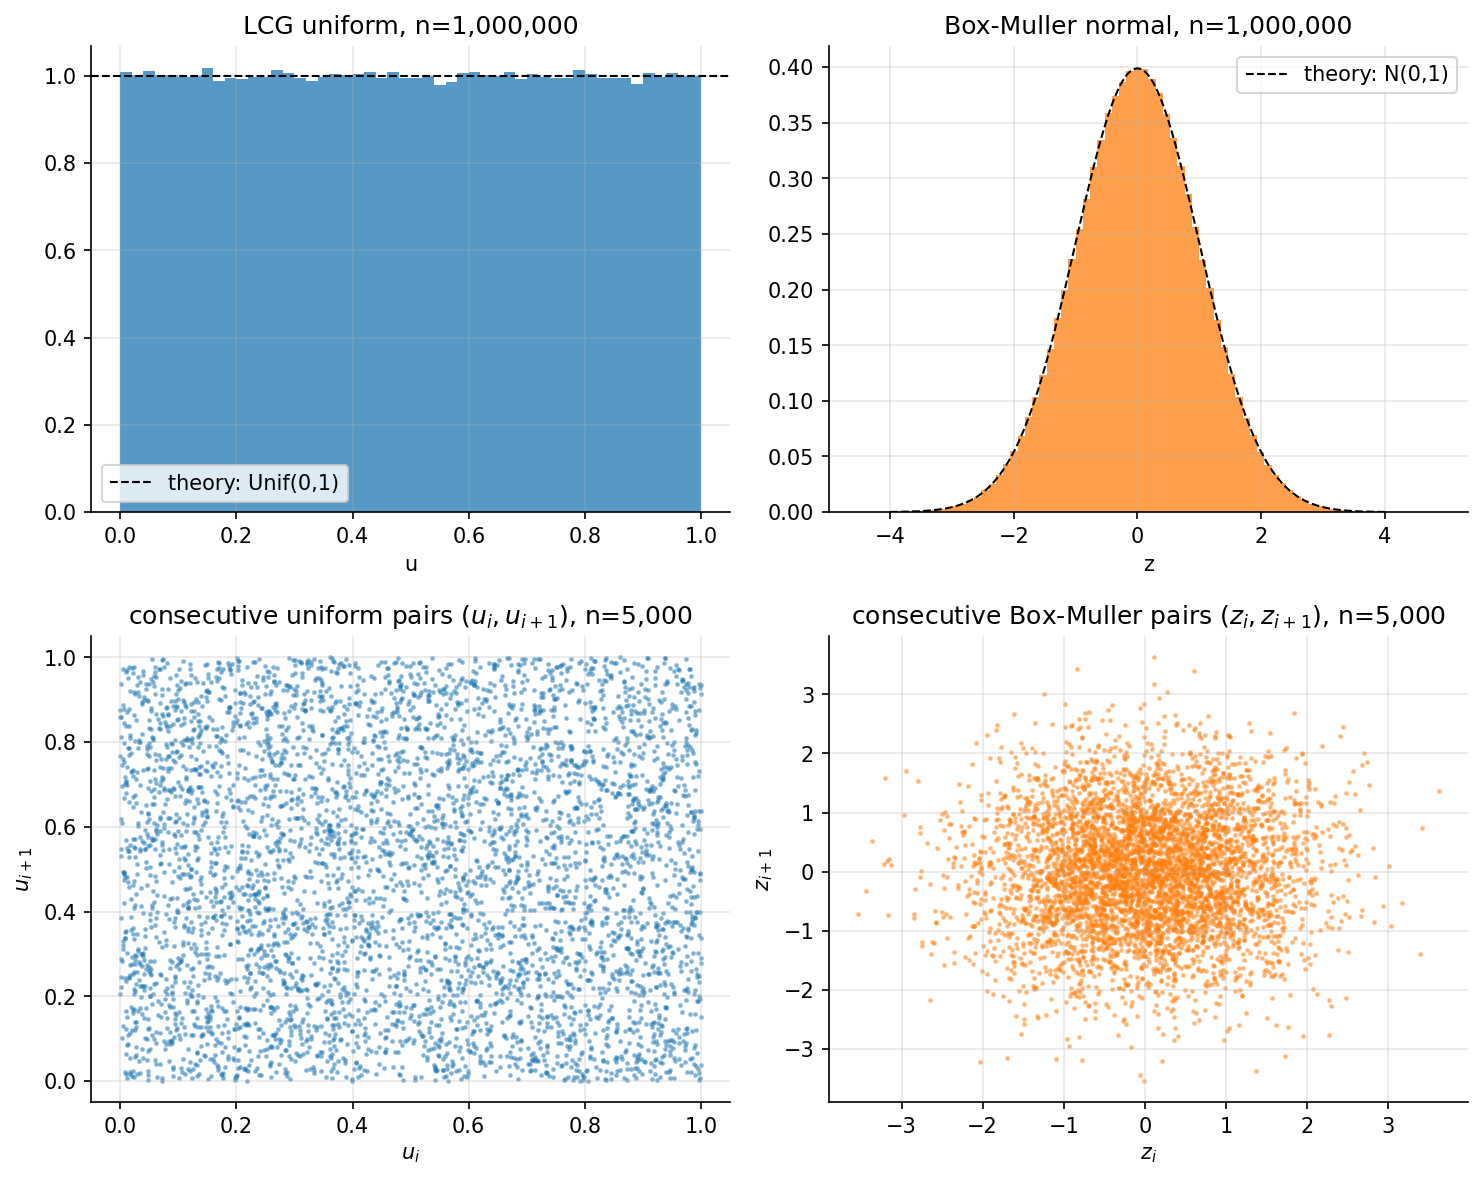
\includegraphics[width=0.72\textwidth]{figures/rng_histograms.png}
  \caption{Top: histograms of $10^6$ LCG uniforms and of $10^6$ Box--Muller normals with the $N(0,1)$ density overlaid. Bottom: 5000 consecutive pairs $(u_i,u_{i+1})$, which fill the unit square uniformly, and 5000 consecutive normal pairs $(z_i,z_{i+1})$, which form a round cloud with no visible structure.}
  \Description{Four panels: a flat uniform histogram, a bell-shaped normal histogram matching the dashed theoretical curve, a uniformly filled scatter plot of consecutive uniform pairs, and a round scatter cloud of consecutive normal pairs.}
  \label{fig:rng}
\end{figure*}

\subsubsection{Forward model}
Table~\ref{tab:threeway} breaks the three-way agreement down by region. The closed form agrees with the stiff Radau ODE integration to about $10^{-13}$, with the explicit RK45 integration to about $10^{-11}$, and with our graded-grid Simpson path to about \sci{3}{-10}. Because the three paths share no algebra, an error in the closed-form derivation would have shown up as a disagreement.

\begin{table}[t]
\caption{Maximum relative difference over the 25 frames between the closed form and independent evaluations of $C_T$.}
\label{tab:threeway}
\footnotesize
\setlength{\tabcolsep}{4pt}
\begin{tabular}{lccc}
\toprule
Region & vs Radau & vs RK45 & vs Simpson \\
\midrule
Frontal      & \sci{1.12}{-13} & \sci{6.93}{-12} & \sci{3.18}{-10} \\
Temporal     & \sci{1.73}{-13} & \sci{8.29}{-12} & \sci{3.29}{-10} \\
Occipital    & \sci{9.54}{-14} & \sci{6.03}{-12} & \sci{2.40}{-10} \\
White matter & \sci{1.37}{-13} & \sci{1.42}{-11} & \sci{2.47}{-10} \\
\bottomrule
\end{tabular}
\end{table}

Table~\ref{tab:phi1} shows why $\phi_1$ needs care. The literal formula $(e^x-1)/x$ loses about half its digits by $x=10^{-8}$, is wrong by 11\% at $x=10^{-15}$, and returns 0 instead of 1 (relative error 1) from $x=10^{-16}$ down, while the \texttt{expm1} form is exact to machine precision everywhere. The near-degeneracy sweep in Figure~\ref{fig:neardeg} tests the related case $a+\mu\to0$ in~\eqref{eq:stablekernel}: across the singular point, the closed form and the quadrature agree to \sci{3.06}{-10}, with no spike.

\begin{table}[t]
\caption{Relative error of $\phi_1(x)$ evaluated literally and with \texttt{expm1}.}
\label{tab:phi1}
\small
\begin{tabular}{ccc}
\toprule
$x$ & $(e^x-1)/x$ & \texttt{expm1}$(x)/x$ \\
\midrule
$10^{-4}$  & \sci{4.3}{-13} & 0 \\
$10^{-8}$  & \sci{1.1}{-8}  & 0 \\
$10^{-12}$ & \sci{8.9}{-5}  & 0 \\
$10^{-15}$ & \sci{1.1}{-1}  & 0 \\
$10^{-16}$ & 1.0 & 0 \\
\bottomrule
\end{tabular}
\end{table}

\begin{figure}[t]
  \centering
  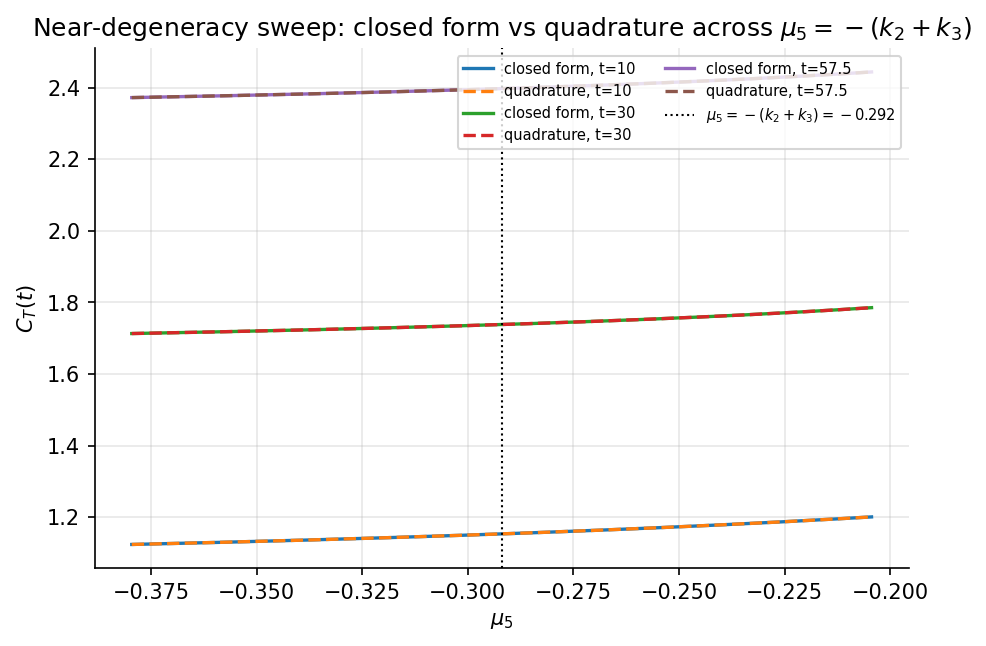
\includegraphics[width=\columnwidth]{figures/near_degeneracy_sweep.png}
  \caption{Closed form and quadrature for $C_T$ at $t=10$, 30 and 57.5 min while one input exponent $\mu_5$ is swept through $-(k_2+k_3)$, where the naive kernel is $0/0$. The curves coincide and stay smooth across the dotted line.}
  \Description{Three pairs of overlapping straight lines, one pair per time point, continuing smoothly across a vertical dotted line at mu5 equal to minus 0.292.}
  \label{fig:neardeg}
\end{figure}

The grid for the quadrature path was chosen by measurement (Table~\ref{tab:grid}). The hardest frame is the last one (57.5 min), because the integral accumulates the most error by then. With a uniform grid ($q=1$), 1601 points leave a relative error of \sci{6.6}{-6} there; the cubic grading $q=3$ reduces it to \sci{3.2}{-10} at the same cost, and at this frame $q=3$ is the best of the gradings $q=1,\dots,5$ at every $n$ we tested.

\begin{table}[t]
\caption{Relative error of the Simpson path at the last frame ($t=57.5$ min) for grids $t_i=t_{\max}u_i^q$.}
\label{tab:grid}
\small
\begin{tabular}{rccc}
\toprule
$n$ & $q=1$ (uniform) & $q=2$ & $q=3$ (adopted) \\
\midrule
401   & \sci{1.17}{-3} & \sci{1.24}{-7}  & \sci{8.12}{-8}  \\
801   & \sci{9.68}{-5} & \sci{7.77}{-9}  & \sci{5.08}{-9}  \\
1601  & \sci{6.56}{-6} & \sci{4.86}{-10} & \sci{3.18}{-10} \\
3201  & \sci{4.18}{-7} & \sci{3.04}{-11} & \sci{1.99}{-11} \\
12801 & \sci{1.64}{-9} & \sci{1.18}{-13} & \sci{7.70}{-14} \\
\bottomrule
\end{tabular}
\end{table}

As an end-to-end use of the QR least-squares routine, we fitted Patlak lines~\cite{patlak1983} to frames 13--25 ($t\ge3.5$ min), plotting $C_T/C_P$ against $\int_0^tC_P\,ds/C_P$ (Figure~\ref{fig:patlak}, Table~\ref{tab:patlak}). The fitted slopes match the classical net influx rate $K_i=K_1k_3/(k_2+k_3)$ to 0.1--1.6\%, with $R^2\ge0.997$. A closer look shows that the classical $K_i$ is itself only approximate for this input. Because the slowest input exponent $\mu_4=-0.0106$ is not negligible, the late-time uptake rate $\dot C_T(t)/C_P(t)$ tends to $K_1(k_3+\mu_4)/(k_2+k_3+\mu_4)$ instead of $K_i$. At the last frame, the classical value is off by 5.6--18.7\%, whereas this corrected value is within 0.05--0.34\%, and at $t=800$ min it is matched to better than \sci{8}{-16}.

\begin{table}[t]
\caption{Patlak slopes fitted with our QR least squares, and the late-time uptake rate $\dot C_T/C_P$ at $t=57.5$ min compared with the classical and corrected formulas.}
\label{tab:patlak}
\footnotesize
\setlength{\tabcolsep}{3.5pt}
\begin{tabular}{lccccc}
\toprule
Region & $K_i$ & slope & $R^2$ & class.\ err. & corr.\ err. \\
\midrule
Frontal      & 0.0634 & 0.0633 & 0.9999 & 5.6\%  & 0.05\% \\
Temporal     & 0.0562 & 0.0561 & 0.9998 & 7.5\%  & 0.08\% \\
Occipital    & 0.0631 & 0.0631 & 0.9996 & 8.2\%  & 0.10\% \\
White matter & 0.0226 & 0.0229 & 0.9970 & 18.7\% & 0.34\% \\
\bottomrule
\end{tabular}
\end{table}

\begin{figure}[t]
  \centering
  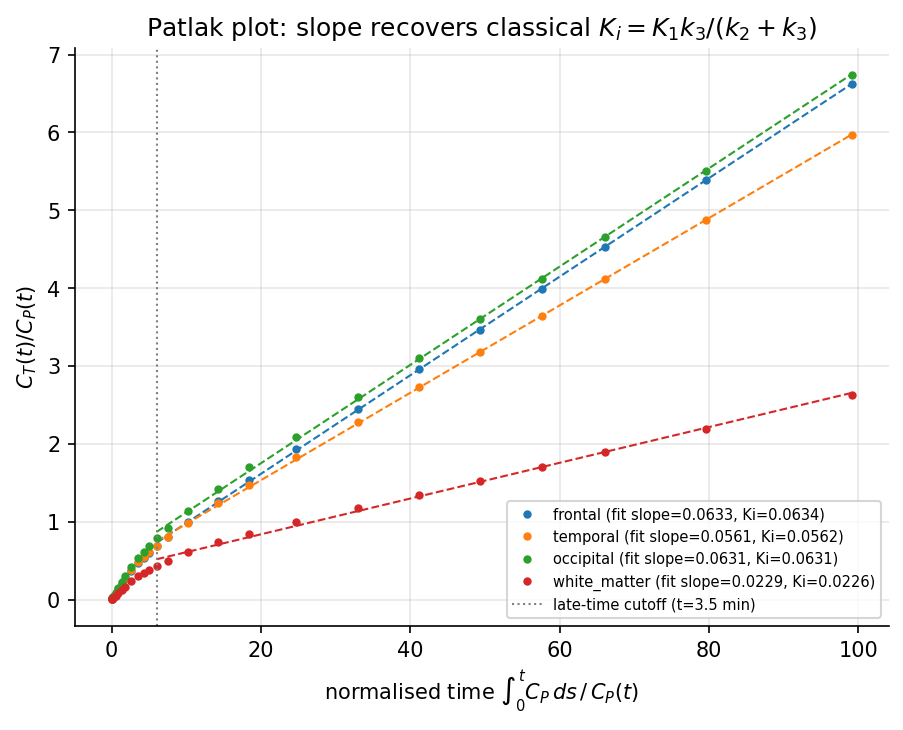
\includegraphics[width=\columnwidth]{figures/patlak_plot.png}
  \caption{Patlak plot for the four regions. Late points (right of the dotted line, $t\ge3.5$ min) fall on straight lines whose QR-fitted slopes recover $K_i$.}
  \Description{Four sets of points rising linearly to the right, with dashed fitted lines; white matter has the smallest slope.}
  \label{fig:patlak}
\end{figure}

\subsubsection{Jacobian, conditioning and noiseless recovery}
The full Jacobian has condition number $7.316\times10^4$. Its normal equations have condition number $5.353\times10^9$, illustrating the expected squaring. Along the regularization schedule, the normal-equation condition number grows from $3.38\times10^2$ to $1.43\times10^{12}$, whereas the stacked QR matrix grows from $18.4$ to $1.20\times10^6$ (Figure~\ref{fig:solvers}). The two paths compute the same step to \sci{2}{-16} at the start, but the gap widens to \sci{5.0}{-10} by the end of the schedule, as the squared condition number predicts. Consequently QR is the production solver.

\begin{figure*}[t]
  \centering
  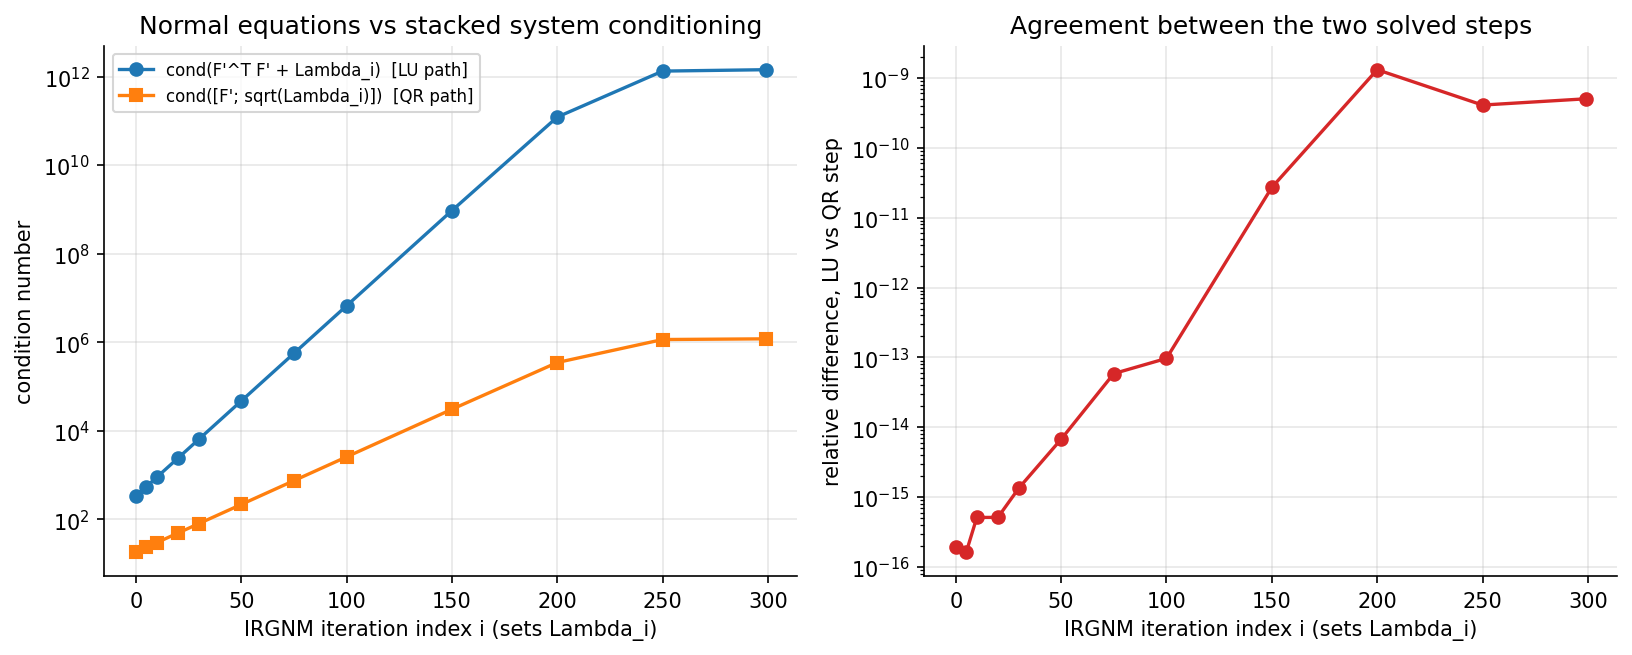
\includegraphics[width=0.86\textwidth]{figures/solver_comparison.png}
  \caption{Left: condition number of the normal-equations matrix (LU path) and of the stacked matrix (QR path) along the IRGNM schedule; the first is roughly the square of the second. Right: relative difference between the steps computed by the two paths.}
  \Description{Left: two rising curves, the blue normal-equations curve reaching about 1e12 and the orange stacked curve about 1e6. Right: a rising red curve from about 1e-16 to about 1e-9.}
  \label{fig:solvers}
\end{figure*}

On the current whole-problem Track A/B check (noiseless tissue and blood data, $\delta_x=0.1$, seed 0), regularized IRGNM reaches relative parameter error $9.27\times10^{-7}$ after 300 iterations in 0.599 s. SciPy's unregularized trust-region least-squares method, given the same residual, analytic Jacobian, and box bounds, terminates after 43 function evaluations in 0.056 s at error 0.094: better than its starting error of 0.301, but about $10^5$ times less accurate than IRGNM. This is not a claim that SciPy is inaccurate: the two optimizers solve differently regularized problems, and the comparison shows why the paper's Tikhonov schedule matters for this ill-posed inverse problem.

The tissue-only Jacobian annihilates the predicted scale direction with norm $9.59\times10^{-17}$ compared with matrix scale $166.1$, and inverse iteration aligns with that direction with cosine 1. Adding the blood block raises the smallest eigenvalue to $4.17\times10^{-6}$. Figure~\ref{fig:conditioning} shows the full spectrum.

\begin{figure}[t]
  \centering
  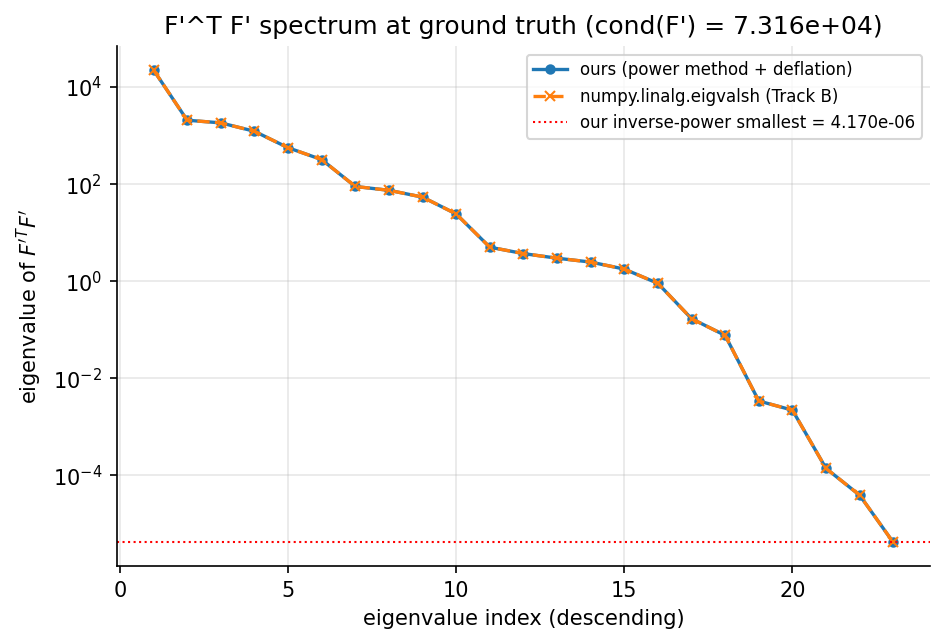
\includegraphics[width=\columnwidth]{figures/conditioning_spectrum.png}
  \caption{Spectrum of $F'^TF'$ at ground truth. Our power/deflation results overlay NumPy's reference; inverse power iteration supplies the smallest eigenvalue.}
  \Description{A logarithmic eigenvalue spectrum decreases from about twenty thousand to four millionths, with hand-written and NumPy curves overlapping.}
  \label{fig:conditioning}
\end{figure}

Noiseless IRGNM recovery from 20 starts per perturbation level produced median relative errors $4.26\times10^{-7}$, $5.21\times10^{-7}$, $5.41\times10^{-7}$, and $9.80\times10^{-7}$ for $\delta_x=0.1,0.2,0.3,0.4$. Divergence counts were 0, 3, 5, and 8 of 20, respectively; no failed trajectory was reseeded away (Table~\ref{tab:recovery}). Figure~\ref{fig:recovery} shows both the characteristic late error decrease and the increasing sensitivity to initialization. In the representative run ($\delta_x=0.1$, seed 0), the data misfit falls by a factor of about 45 in the first 100 iterations while the parameter error barely changes: the solver first fixes the directions the data constrain strongly, and only later the nearly flat directions identified by the conditioning analysis.

\begin{table}[t]
\caption{Noiseless IRGNM recovery, 20 seeds per perturbation level, 300 iterations. ``Clipped'' counts starts that had to be projected into the feasible box.}
\label{tab:recovery}
\footnotesize
\begin{tabular}{ccccc}
\toprule
$\delta_x$ & diverged & clipped & median error & mean iter. \\
\midrule
0.1 & 0/20 & 0 & \sci{4.26}{-7} & 300.0 \\
0.2 & 3/20 & 0 & \sci{5.21}{-7} & 276.1 \\
0.3 & 5/20 & 2 & \sci{5.41}{-7} & 267.6 \\
0.4 & 8/20 & 3 & \sci{9.80}{-7} & 249.3 \\
\bottomrule
\end{tabular}
\end{table}

\begin{figure*}[t]
  \centering
  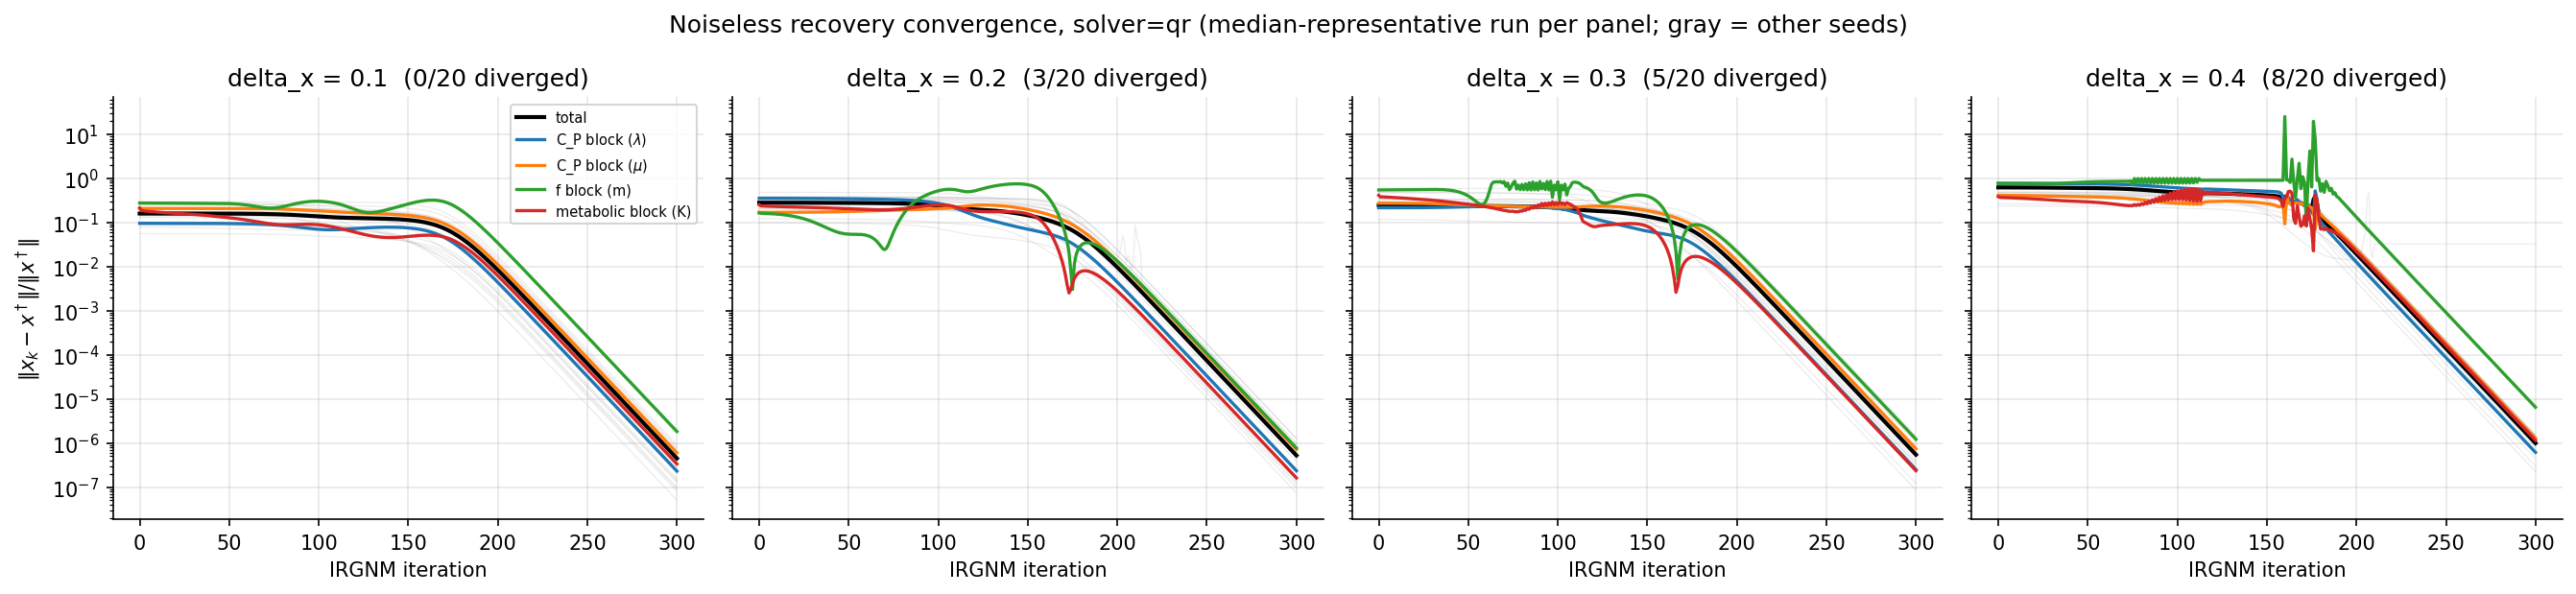
\includegraphics[width=0.98\textwidth]{figures/noiseless_recovery_qr.png}
  \caption{Noiseless IRGNM convergence. Colored curves are blockwise errors for a representative successful run; gray curves show other seeds.}
  \Description{Four panels show logarithmic parameter errors over 300 iterations for increasing initial perturbation, with more divergence at larger perturbations.}
  \label{fig:recovery}
\end{figure*}

\subsection{Identifiability signature}

Table~\ref{tab:identifiability} is the central result. Across 65 accepted tissue-only fits, the common-ratio spread never exceeds $1.83\times10^{-8}$ even though $\zeta$ ranges from 0.693 to 2.269 and the largest $K_1$ relative error is 127\%. In the same fits, the maximum $k_2$ and $k_3$ errors are only $1.33\times10^{-6}$ and $5.11\times10^{-7}$. This separation is direct numerical evidence for the paper's structural theorem, rather than merely a successful curve fit.

\begin{table*}[t]
\caption{Noiseless tissue-only identifiability and removal by one early $C_P$ measurement. The spread is $\max_i r_i/\min_i r_i-1$, $r_i=K_{1,\mathrm{est}}^i/K_{1,\mathrm{true}}^i$.}
\label{tab:identifiability}
\small
\begin{tabular}{cccccccc}
\toprule
$\delta_x$ & Accepted/20 & $\zeta$ range & Worst spread & Max $K_1$ error & Max $k_2$ error & Max $k_3$ error & One $C_P$: max $|\zeta-1|$ \\
\midrule
0.1 & 18 & 0.838--1.335 & $7.59\times10^{-9}$ & 0.335 & $5.68\times10^{-7}$ & $2.19\times10^{-7}$ & $7.65\times10^{-8}$ \\
0.2 & 17 & 0.697--1.472 & $1.83\times10^{-8}$ & 0.472 & $1.33\times10^{-6}$ & $5.03\times10^{-7}$ & $1.37\times10^{-7}$ \\
0.3 & 17 & 0.693--1.862 & $1.77\times10^{-8}$ & 0.862 & $1.32\times10^{-6}$ & $5.11\times10^{-7}$ & $1.73\times10^{-7}$ \\
0.4 & 13 & 0.754--2.269 & $1.52\times10^{-8}$ & 1.269 & $1.15\times10^{-6}$ & $4.45\times10^{-7}$ & $1.37\times10^{-7}$ \\
\bottomrule
\end{tabular}
\end{table*}

The best single sample occurs at $t=0.2917$ min, where $C_P=4.7995$; late samples at 15 and 57.5 min are 20--60 times less effective. Under the full-step RMS convention, tissue-only median spreads are about 0.49--0.54\% at high count and 1.76--1.96\% at normal count, while $\zeta$ still varies substantially. At low count only 2 of 80 tissue-only fits are accepted, so the signature is no longer distinguishable. Adding one early $C_P$ sample yields median $|\zeta-1|$ of 0.66--0.79\% at high count and 2.47--3.02\% at normal count, but no accepted low-count fits. Correct Morozov early stopping improves estimation stability but masks the asymptotic ratio coincidence because it stops before the iterate fully settles onto the null manifold.

\subsection{Noise, consistency, and regularization}

The calibrated Poisson noise produced mean RMS discrepancies $0.002958\pm0.000261$, $0.011616\pm0.001076$, and $0.070341\pm0.006409$ for high, normal, and low count. In the controlled consistency experiment with one exact early plasma sample and $\delta_x=0.1$, mean kinetic error decreases from $0.14430\pm0.04052$ at normal count to $0.12109\pm0.04940$ at high count and to $(1.97\pm1.04)\times10^{-7}$ without noise. All 20 low-count cases stop at iteration zero, correctly indicating that the data do not justify moving away from the initial guess.

Regularization reduces the sum of truth-normalized fitted-parameter variances from 0.28668 to 0.16263 at high count (factor 1.76) and from 1.35754 to 0.30952 at normal count (factor 4.39), measured on 14 paired successful seeds in each level. A fixed-Jacobian one-step diagnostic, which retains all 20 paired observations, gives still larger variance-reduction factors of 2231, 1251, and 420 for high, normal, and low count. Figure~\ref{fig:consistency} summarizes both checks.

\begin{figure*}[t]
  \centering
  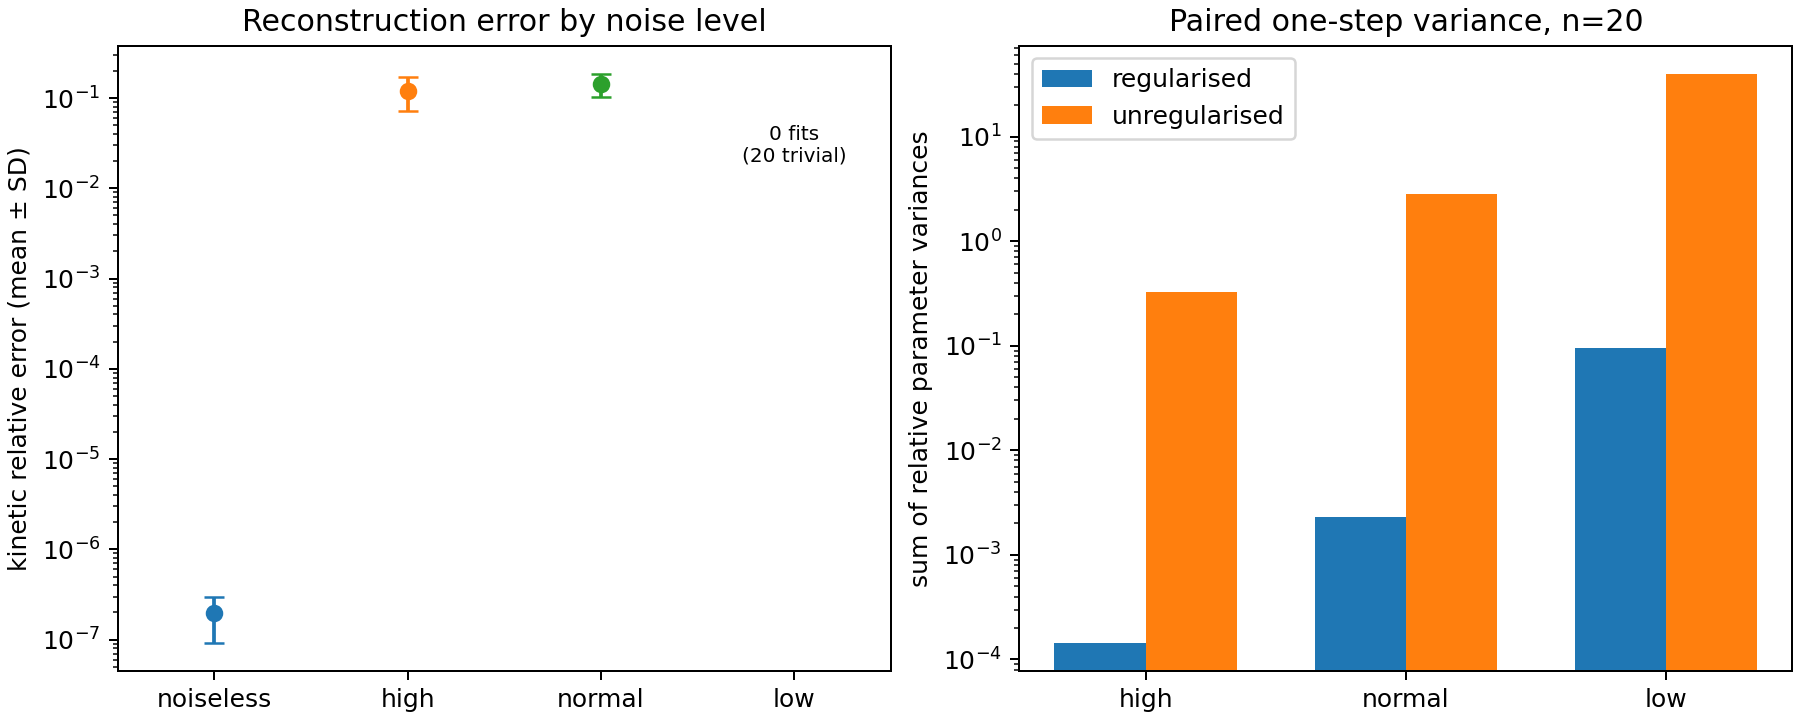
\includegraphics[width=0.92\textwidth]{figures/consistency_regularization.png}
  \caption{Left: kinetic reconstruction error decreases with the noise level; low count yields only trivial stops. Right: paired one-step parameter variance with and without regularization.}
  \Description{The left logarithmic plot shows near-zero noiseless error and about one-tenth error for high and normal count. The right bar chart shows much larger unregularized variance at every noise level.}
  \label{fig:consistency}
\end{figure*}

\subsection{Monte Carlo trends and comparison with the paper}

The original 960-cell grid records 494 non-finite divergences: 28 noiseless, 76 high-count, 153 normal-count, and 237 low-count. Thus failure probability grows sharply with noise; Figure~\ref{fig:figure7} shows typical noisy trajectories. Among finite M4.3 runs, mean per-seed $K_1$ versus $k_3$ relative errors are 0.0106 versus 0.1576 in Setup B and 0.0160 versus 0.0850 in Setup C, agreeing with the paper that $K_1$ is generally easier to recover. Setup A reverses the ordering (0.2307 versus 0.1737), as expected because it deliberately removes arterial data and exposes the $K_1/\lambda$ ambiguity.

For $\delta_x=0.1$, known $C_P$ beats clean $C_{WB}$ at both high count (0.1211 vs 0.1324 kinetic error) and normal count (0.1443 vs 0.4149). Clean $C_{WB}$ beats noisy $C_{WB}$ at high count (0.1324 vs 0.1668) but reverses at normal count (0.4149 vs 0.3582), where only 7 runs per cell survive. We therefore classify that comparison as mixed rather than smoothing over the small-sample result.

The original grid uses a stopping rule with a scaling error and a single set of solver settings for all setups. Section~\ref{sec:improvements} reruns it with each correction in turn: with the paper's own settings, failure counts match the paper at high and normal count, and the remaining mismatch is concentrated in low count and noiseless distant starts. At low count, direct TAC noise often makes the discrepancy bound larger than the starting residual, producing a valid iteration-zero stop rather than a solver blow-up. These results support qualitative, not digit-for-digit, agreement; Table~\ref{tab:trends} lists each predicted trend with its verdict.

\begin{table}[t]
\caption{Predicted trends and measured verdicts.}
\label{tab:trends}
\small
\begin{tabular}{p{0.42\columnwidth}p{0.48\columnwidth}}
\toprule
Trend & Verdict and evidence \\
\midrule
$K_1$ easier than $k_3$ & Agrees in B/C; A reverses as Proposition 12 predicts \\
Known $C_P$ better than clean $C_{WB}$ & Agrees at high and normal count \\
Clean $C_{WB}$ better than noisy $C_{WB}$ & High agrees (14 and 13 survivors); normal reverses (7 each) \\
Low count fails & Agrees: 237/240 grid fits diverge \\
Regularization lowers variance & Agrees: factors 1.76 and 4.39 in full fits \\
Few failures (paper's settings) & Agrees at high and normal count (14 vs 19, 18 vs 35); differs at low count and without noise \\
\bottomrule
\end{tabular}
\end{table}

\begin{figure*}[t]
  \centering
  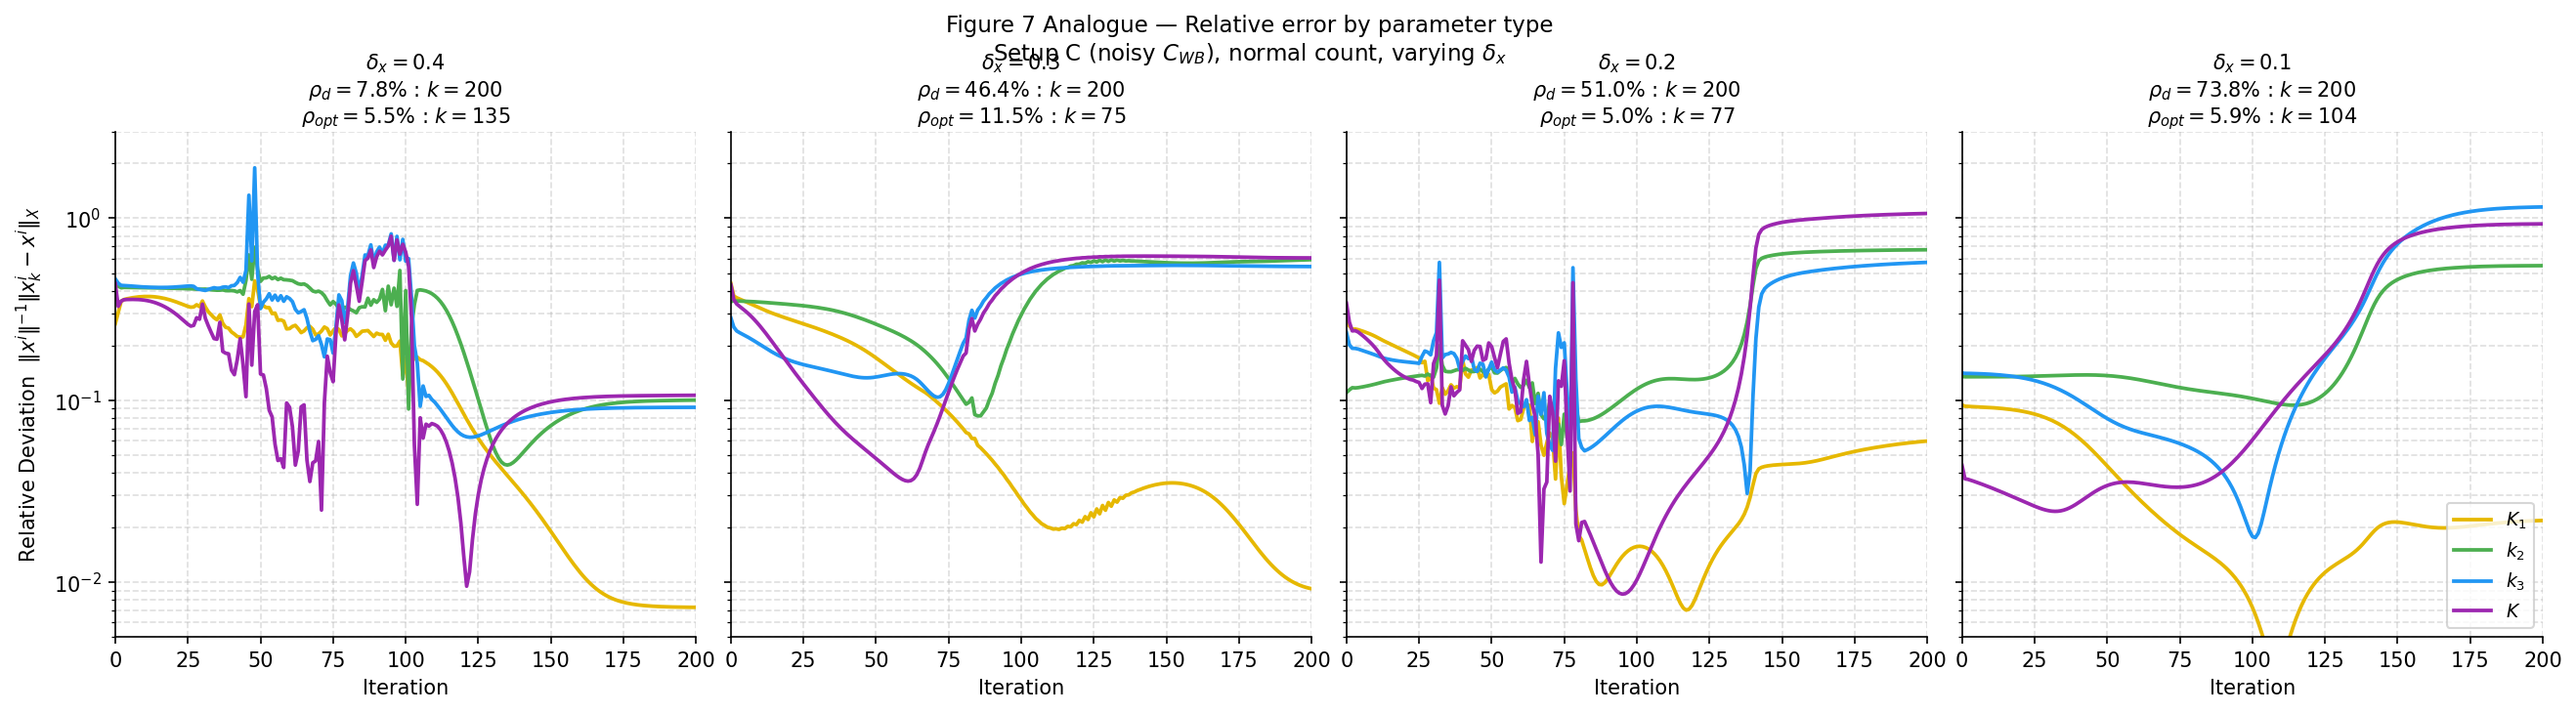
\includegraphics[width=0.98\textwidth]{figures/figure7_analogue.png}
  \caption{Current Figure~7 analogue for Setup C at normal count. Each panel shows the relative deviation of $K_1$, $k_2$, $k_3$, and the combined kinetic block for one initialization level. The printed iteration and residual annotations expose early improvement followed by noise fitting or instability.}
  \Description{Four panels show logarithmic parameter-error trajectories for noisy whole-blood fitting at four initial perturbation levels.}
  \label{fig:figure7}
\end{figure*}

\begin{table*}[t]
\caption{Numerical enhancements tried during the project, the problem each addressed, and the measured outcome.}
\label{tab:enhancements}
\small
\begin{tabular}{p{0.21\textwidth}p{0.29\textwidth}p{0.33\textwidth}p{0.09\textwidth}}
\toprule
Enhancement & Problem addressed & Measured outcome & Status \\
\midrule
Partial pivoting in LU & division by small pivots amplifies rounding & residual $\le\sci{4.7}{-16}$ on 200 systems & adopted \\
Householder sign choice & cancellation in $x_1-\alpha$ & QR residual $\le\sci{9.2}{-16}$ & adopted \\
Stacked QR instead of normal equations & $\kappa(F'^TF'+\Lambda)\approx\kappa(\text{stacked})^2$ & condition \sci{1.20}{6} instead of \sci{1.43}{12} & adopted \\
Simpson on nonuniform grids & PET frames and graded grids are not uniform & orders 3.9987--4.0125 measured & adopted \\
Local-coordinate Simpson weights & cancellation in cubic antiderivatives & floor \sci{2.10}{-10} (n=513) replaced by \sci{6.62}{-14} (n=2001) & adopted \\
Graded grid $t=t_{\max}u^3$, $n=1601$ & early bolus needs dense sampling & last-frame error \sci{3.18}{-10} vs \sci{6.56}{-6} uniform & adopted \\
\texttt{expm1}-based $\phi_1$ & $0/0$ and cancellation at small $x$ & relative error 0 vs 1.0 at $x\le10^{-16}$ & adopted \\
Taylor series for $\phi_2$ below $10^{-4}$ & cancellation persists in $e^x-1-x$ & threshold measured; Jacobian agrees with finite differences & adopted \\
Factored kernel~\eqref{eq:stablekernel} & $0\cdot\infty$ and $a+\mu\to0$ & smooth across the singular point, \sci{3.06}{-10} & adopted \\
Poisson crossover at $\lambda=30$ & $O(\lambda)$ cost; endless loop for $\lambda\gtrsim745$ & mean and variance within Monte Carlo error up to $\lambda=1000$ & adopted \\
Seed mixing and derived seeds & related streams from nearby seeds & identical streams across processes & adopted \\
Corrected late-time slope & classical $K_i$ ignores the slowest input exponent & error 5.6--18.7\% reduced to 0.05--0.34\% & analysis \\
Blockwise regularization & parameters span a scale ratio of 2690 & noiseless recovery to $\approx10^{-6}$ & adopted \\
Corrected Morozov scale & RMS vs 2-norm mismatch in the stopping rule & non-finite failures 494 reduced to 58 (Table~\ref{tab:improvement-effects}) & adopted \\
Paper's per-setup settings & one setting used for all three setups & failures match the paper at high and normal count & adopted \\
Armijo line search & divergence from distant starts & same result on the reference fit; grid not yet evaluated & opt-in \\
\bottomrule
\end{tabular}
\end{table*}

\begin{table*}[t]
\caption{Course topics used in the project.}
\label{tab:course}
\small
\begin{tabular}{p{0.20\textwidth}p{0.30\textwidth}p{0.43\textwidth}}
\toprule
Topic & Implementation & Produced evidence \\
\midrule
Round-off/truncation error & \texttt{phi1}, \texttt{phi2} series, stable moments, local Simpson weights & Table~\ref{tab:phi1}; translated-quadratic and fine-grid study \\
Condition number and ill-conditioning & Hilbert stress test; Jacobian spectrum & Table~\ref{tab:hilbert}: about $\log_{10}\kappa$ digits lost; $\kappa(F')=\sci{7.3}{4}$ \\
Bisection root finding & \texttt{calibrate\_poisson}, \texttt{calibrate\_gaussian} & noise targets reached by log-scale bisection \\
LU/Gaussian elimination & \texttt{src/linalg.py}, Algorithm~\ref{alg:lu} & $6.48\times10^{-16}$ max error over 200 systems \\
Householder QR & \texttt{src/qr.py}, Algorithm~\ref{alg:qr} & stacked IRGNM solve and all log--log regressions \\
Power method & \texttt{src/eigen.py} & Jacobian conditioning spectrum and smallest eigenvalue \\
Random-number generation & \texttt{src/rng.py} & Table~\ref{tab:rng}: moments, $\chi^2$, autocorrelation, Poisson \\
Monte Carlo simulation & \texttt{src/montecarlo.py} & 960-cell seeded noise/initialization grid \\
Newton-type optimization & \texttt{src/irgnm.py} & regularized Gauss--Newton recovery and constraints \\
Least-squares regression & \texttt{src/qr.lstsq}; Patlak experiment~\cite{patlak1983} & Table~\ref{tab:patlak}: late-time Patlak $R^2=0.9970$--$0.9999$ \\
Newton--Cotes integration & \texttt{trapezoid}, \texttt{simpson} & Table~\ref{tab:quadratio}: second- and fourth-order convergence \\
Numerical differentiation & central-difference benchmark & independent analytic-Jacobian verification \\
\bottomrule
\end{tabular}
\end{table*}

\subsection{Effect of the improvements}
\label{sec:improvements}

Each improvement was evaluated by rerunning the same seeded experiments with only that change switched on, so the before-and-after values in Table~\ref{tab:improvement-effects} share observations, initial guesses, and seeds. The base paper's published settings were used exactly; nothing was tuned to match its results.

\begin{table*}[!t]
\caption{Effect of each improvement on the measured results. Monte Carlo rows use the full 960-fit grid; ``no improvement'' is the paper's failure criterion (final error not below the initial error).}
\label{tab:improvement-effects}
\small
\begin{tabular}{p{0.26\textwidth}p{0.34\textwidth}p{0.13\textwidth}p{0.17\textwidth}}
\toprule
Improvement & Measured quantity & Before & After \\
\midrule
Corrected stopping-rule scale, 200-step cap & Monte Carlo blow-ups (non-finite) & 494 & 58 \\
 & Monte Carlo ``no improvement'' & 512 & 172 \\
Paper's per-setup settings and reduced setup & Monte Carlo blow-ups & 58 & 43 \\
 & Monte Carlo ``no improvement'' (paper: 97) & 172 & 222 \\
Blood readings at all 25 frames (not adopted) & Monte Carlo blow-ups / ``no improvement'' & 43 / 222 & 84 / 209 \\
Local-coordinate Simpson weights & Simpson error, $\int_0^\pi\sin x\,dx$, $n=12801$ & \sci{1.8}{-7} & \sci{1.3}{-15} \\
 & PET forward model, max relative error, $n=12801$ & \sci{1.27}{-7} & \sci{7.99}{-14} \\
Stable exponential kernels & Quadrature vs Radau, $n=1601$ & \sci{5.88}{-10} & \sci{3.29}{-10} \\
 & SciPy least-squares final error (reference fit) & 1.046 & 0.094 \\
 & IRGNM final error (reference fit) & \sci{9.27}{-7} & \sci{9.27}{-7} \\
Armijo line search (opt-in) & IRGNM final error (reference fit) & \sci{9.27}{-7} & \sci{9.27}{-7} \\
\bottomrule
\end{tabular}
\end{table*}

\begin{table}[!htb]
\caption{Failure counts against the paper's Table~1 under its ``no improvement'' criterion, out of 240 fits per noise level.}
\label{tab:failure-counts}
\small
\begin{tabular}{lccc}
\toprule
Noise & Paper & Original & Paper's settings \\
\midrule
Noiseless & 1 & 28 & 29 \\
High count & 19 & 78 & 14 \\
Normal count & 35 & 167 & 18 \\
Low count & 42 & 239 & 161 \\
\midrule
Total & 97 & 512 & 222 \\
\bottomrule
\end{tabular}
\end{table}

The stopping-rule correction accounts for most of the change. The original code compared an RMS noise level with the 2-norm of the residual, which made the discrepancy principle $\sqrt{100}=10$ times too strict, so noisy runs never stopped early and many diverged. With the paper's settings (Table~\ref{tab:failure-counts}), failure counts at high and normal count match the paper (14 vs 19, 18 vs 35). The paper's settings raise the ``no improvement'' total from 172 to 222 because its larger stopping constants ($\tau=9.2$ and 17.6) stop more low-count runs at once: 158 of the 161 low-count failures stop at iteration zero, where $\tau\delta$ already exceeds the initial residual, and none diverges. These are a consequence of adding noise directly to the TACs, not solver breakdowns. The remaining unexplained gap is noiseless: 29 of 240 runs from the most distant starts fail, against 1 in the paper. The stability changes left IRGNM's reference result unchanged but improved SciPy's from 1.046 to 0.094, because both solvers now receive more accurate model values; IRGNM remains about $10^5$ times more accurate.

\subsection{Floating-point stability and performance}

The local-coordinate Simpson formulation removes a coordinate-dependent arithmetic defect. Translating the same quadratic samples by $10^3$ changes the legacy error from $8.88\times10^{-16}$ to $6.36\times10^{-7}$, while the local formula remains exact at float64 precision. On all PET regions and frames, increasing the graded grid to 12,801 points reduces maximum error to $7.99\times10^{-14}$ with local weights, whereas the legacy formulation rises to $1.27\times10^{-7}$. Figure~\ref{fig:simpson} shows that algebraically equivalent formulas need not be numerically equivalent.

\begin{figure*}[t]
  \centering
  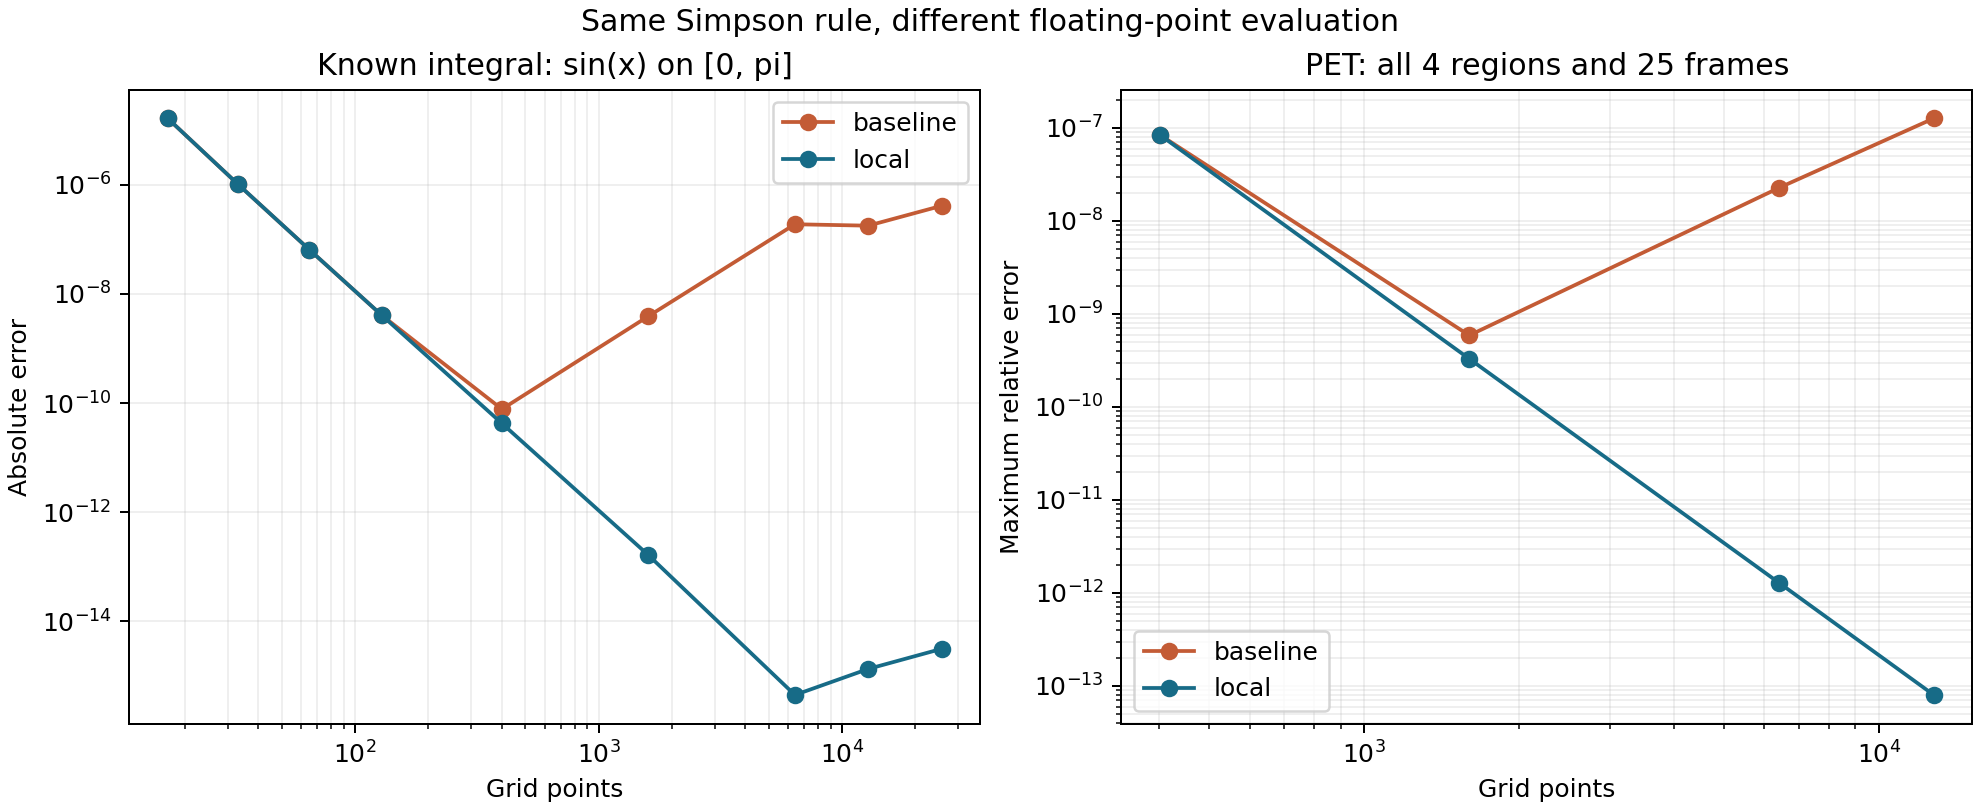
\includegraphics[width=0.92\textwidth]{figures/simpson_local_convergence.png}
  \caption{The same Simpson rule evaluated with legacy absolute-coordinate weights and stable local-coordinate weights. Local evaluation removes the fine-grid round-off growth.}
  \Description{Two logarithmic plots compare baseline and local-coordinate Simpson errors; the local method continues toward machine precision while the baseline rises on fine grids.}
  \label{fig:simpson}
\end{figure*}

Operation-count expectations and measured timing tell different stories at small sizes. LU and square QR are cubic in theory, but fitted exponents over $n=20$--100 are 1.22 and 1.16 because interpreter and dispatch overhead dominate. The IRGNM stacked least-squares solve, measured over 23--736 columns, has exponent 2.60, closer to the cubic count. Simpson is linear and measures exponent 1.02 over 101--25,601 points. At the fixed physical problem size, the recorded IRGNM run averages 1.96 ms per iteration. Figure~\ref{fig:timing} shows the fits. Track B is faster because it uses optimized compiled kernels; its purpose here is validation, not replacement of the required hand-written algorithms.

\begin{figure*}[t]
  \centering
  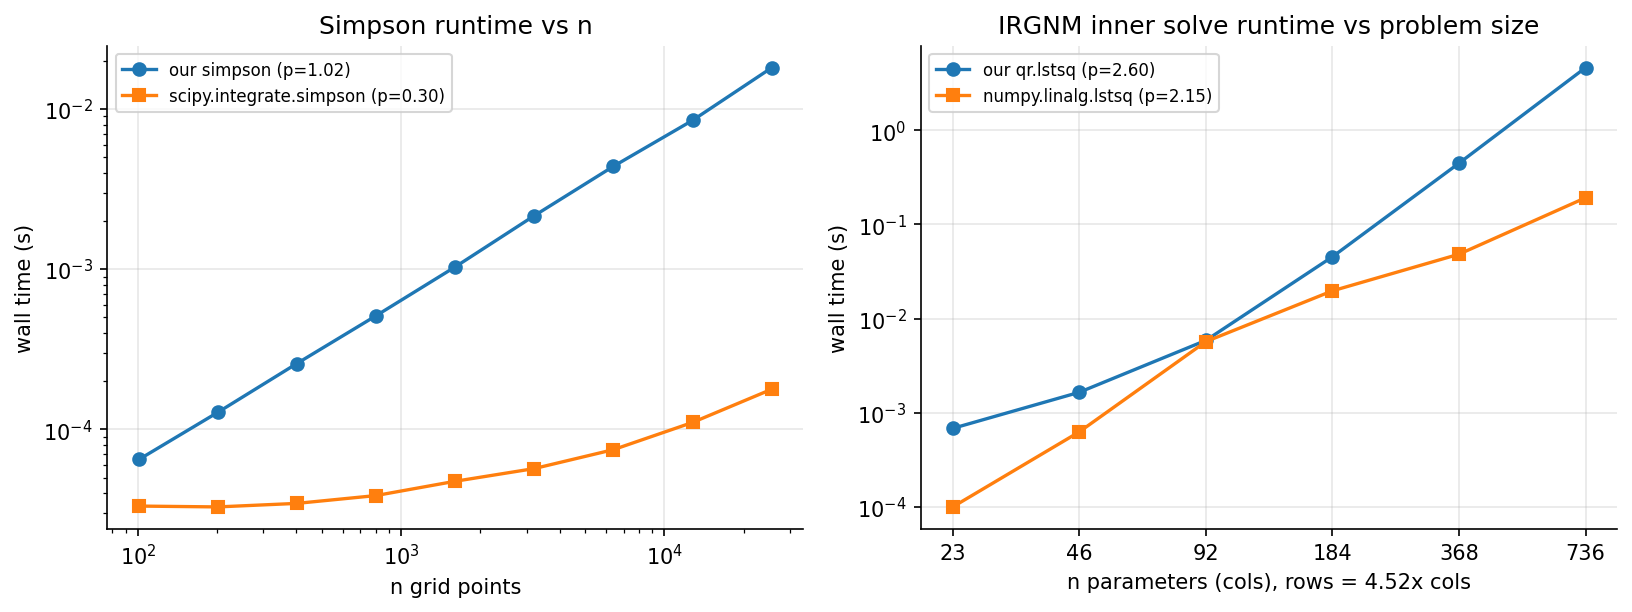
\includegraphics[width=0.90\textwidth]{figures/timing_complexity.png}
  \caption{Measured scaling of Simpson integration and the stacked least-squares solve used inside IRGNM. Timing constants are machine-dependent; slopes are fitted by our QR least-squares implementation.}
  \Description{Two log-log plots compare hand-written and library runtimes as integration grid size and least-squares problem size increase.}
  \label{fig:timing}
\end{figure*}

\subsection{Enhancements and design iterations}

Several choices in the final pipeline replaced a simpler first version after a measurement showed a problem. Table~\ref{tab:enhancements} lists them with the evidence that motivated each one, including one enhancement that was implemented but not yet evaluated. Two of them deserve comment. First, our first Simpson implementation integrated each quadratic through differences of cubic antiderivatives in absolute coordinates. Its error stopped improving at $n=513$ (\sci{2.10}{-10} for $\sin x$) and then grew to \sci{4.81}{-9} at $n=2001$. Rewriting the same weights in local coordinates~\eqref{eq:simpson} removed this floor: the error now keeps falling to \sci{6.62}{-14}. Second, the Armijo backtracking line search accepts a step only if it decreases the regularized objective sufficiently, and falls back to a scaled projected-gradient direction when projection destroys descent. It targets the divergences from distant starts in Table~\ref{tab:recovery}. It is merged into the solver as an opt-in flag, off by default. On the reference noiseless fit it accepts the full step every time and reaches the same $9.27\times10^{-7}$, but it has not been run through the recovery study or the Monte Carlo grid, so we make no claim about its effect on divergence.

\subsection{Course-topic mapping}

Table~\ref{tab:course} maps the relevant CSE 402 topics to concrete code and evidence. Methods not required by this inverse problem, such as Bairstow, golden-section search, Romberg integration, and interpolation of tabulated solutions, were not inserted artificially.

\section{Conclusion and Future Work}

This project reproduces the base paper's central identifiability phenomenon with an independently implemented numerical stack. The strongest result is not simply low fitting error: without arterial data, four independently parameterized regions return $K_1$ ratios agreeing to $1.83\times10^{-8}$ while $K_1$ itself may be wrong by 127\%, and one early plasma sample collapses the scale error to at most $1.73\times10^{-7}$. Correcting the stopping-rule scale and using the paper's per-setup settings reduced Monte Carlo blow-ups from 494 to 43 and brought the high- and normal-count failure counts in line with the paper. Every primitive underneath that result was verified on its own: LU and QR at the round-off level, Simpson at its theoretical order, the random generators against their target distributions, and the forward model against two independent integrators. The Jacobian, conditioning analysis, and noiseless IRGNM recovery are also independently verified. The noisy experiments show both the benefit of regularization and the limits of low-count data.

The study has four main limitations. First, TAC-level noise is not a substitute for sinogram generation and OSEM reconstruction, so absolute divergence counts cannot be compared directly with the paper. Second, nonlinear convergence remains sensitive to distant initial guesses: 8 of 20 noiseless runs diverge at $\delta_x=0.4$, 29 of 240 noiseless grid runs fail against 1 in the paper, and the default solver takes full steps; an Armijo-globalized option is implemented but not yet evaluated. Third, the normal approximation used for large-rate Poisson draws is efficient but approximate. Fourth, all data are synthetic and use one fixed four-region model.

Future work should evaluate the Armijo-globalized IRGNM that is already implemented, reproduce the scanner/reconstruction chain, evaluate exact or rejection-based large-rate Poisson samplers, optimize blood-sample timing under noise, and test the method on realistic or clinical TACs. Pinning the complete numerical environment and packaging the report build into the one-command runner would further strengthen reproducibility.

\begin{acks}
The project was completed for CSE 402: Numerical Analysis, Simulation and Modeling at Bangladesh University of Engineering and Technology. The authors thank the course instructors for the project framework.
\end{acks}

\bibliographystyle{ACM-Reference-Format}
\bibliography{references}

\end{document}
